%==============================================================================
%  MAJOR PROJECT-I REPORT  --  Adani Institute of Higher Education and Research (DU)
%  Project: Vision-Based Defect Detection System for Industrial Quality Inspection
%  Student: Nakul S. Dube (Enrollment No.: C2023FE00055 / DMET1323009)
%  Supervisor: Dr. Utkarsha Pacharaney
%  Compile with:  pdflatex main  ->  bibtex main  ->  pdflatex main  (x2)
%  (or simply use latexmk -pdf main.tex ; on Overleaf just press "Recompile")
%==============================================================================
\documentclass[12pt,a4paper]{report}

% ---------- Page geometry (standard thesis margins) ----------
\usepackage[a4paper,left=1.25in,right=1in,top=1in,bottom=1in]{geometry}

% ---------- Fonts: Times New Roman look-alike, 12 pt, 1.5 spacing, justified ----------
\usepackage[T1]{fontenc}
\usepackage[utf8]{inputenc}
\usepackage{mathptmx}
\usepackage[expansion=false]{microtype}
\usepackage{setspace}
\onehalfspacing
\usepackage{ragged2e}          % \justifying inside table cells

% ---------- Graphics, colour, tables, lists ----------
\usepackage{graphicx}
\usepackage[table]{xcolor}
\usepackage{amsmath,amssymb}
\usepackage{booktabs,longtable,array,multirow,makecell,tabularx}
\usepackage{enumitem}
\usepackage{float}
\usepackage{caption}
\usepackage{subcaption}
\usepackage{tikz}
\usetikzlibrary{shapes.geometric,arrows.meta,positioning,calc,fit}
\usepackage[ruled,vlined,linesnumbered]{algorithm2e}
\usepackage{titlesec}
\usepackage{tocloft}
\usepackage{cite}
\usepackage[colorlinks=true,linkcolor=black,citecolor=black,urlcolor=blue!50!black]{hyperref}
\usepackage[nottoc]{tocbibind}

% ---------- Captions: "Figure 2.1: ..." / "Table 3.1: ..." ----------
\captionsetup{labelsep=colon,font={small,stretch=1},skip=6pt}
\setlength{\textfloatsep}{12pt plus 2pt minus 2pt}

% ---------- Headings: Chapter N / Title (centred), 1.1, 1.1.1 ----------
\setcounter{secnumdepth}{3}
\setcounter{tocdepth}{2}
\titleformat{\chapter}[display]{\normalfont\bfseries\centering}
  {\fontsize{16}{20}\selectfont Chapter \thechapter}{4pt}{\fontsize{20}{24}\selectfont}
\titleformat{name=\chapter,numberless}[display]{\normalfont\bfseries\centering}
  {}{0pt}{\fontsize{20}{24}\selectfont}
\titlespacing*{\chapter}{0pt}{0pt}{22pt}
\titleformat{\section}{\normalfont\Large\bfseries}{\thesection}{0.8em}{}
\titleformat{\subsection}{\normalfont\large\bfseries}{\thesubsection}{0.8em}{}
\titleformat{\subsubsection}{\normalfont\normalsize\bfseries\itshape}{\thesubsubsection}{0.8em}{}
\titlespacing*{\section}{0pt}{16pt}{8pt}
\titlespacing*{\subsection}{0pt}{12pt}{6pt}
\titlespacing*{\subsubsection}{0pt}{10pt}{4pt}

% ---------- Paragraphs ----------
\setlength{\parindent}{0pt}
\setlength{\parskip}{6pt plus 1pt}
\setlist{itemsep=2pt,topsep=4pt,parsep=0pt}
\renewcommand{\bibname}{References}

% ---------- Project-wide macros ----------
\newcommand{\ProjectTitle}{VISION-BASED DEFECT DETECTION SYSTEM FOR INDUSTRIAL QUALITY INSPECTION}
\newcommand{\ProjectTitleCase}{Vision-Based Defect Detection System for Industrial Quality Inspection}
\newcommand{\StudentName}{Nakul S. Dube}
\newcommand{\Enrollment}{C2023FE00055}
\newcommand{\EnrollmentTitle}{DMET1323009}
\newcommand{\SupervisorName}{Dr.\ Utkarsha Pacharaney}
\newcommand{\CoordinatorName}{Dr.\ Subodh Daronde}
\newcommand{\HODName}{Dr.\ Utkarsha Pacharaney}
\newcommand{\DeanAcademics}{Dr.\ Utkarsha Pacharaney}
\newcommand{\DeanFEAT}{Prof.\ (Dr.)\ K.T.V.\ Reddy}
\newcommand{\DeptName}{Artificial Intelligence and Machine Learning}
\newcommand{\UniversityName}{Adani Institute of Higher Education and Research (DU)}
\newcommand{\code}[1]{\texttt{\detokenize{#1}}}

\begin{document}

% Ensure all 30 references are included and numbered [1] to [30] sequentially
\nocite{wang2024rgs, terven2023yolo, chen2025obb, huang2026msfe, li2024pv, zhang2025msf, sun2023ds, yang2024gradient, cheng2024efen, patel2023deep, xu2025sfc, zhao2024rst, deng2024probiou, meng2024automated, zhou2024lska, jiang2024realtime, song2025multiangle, liu2024dmd, wang2024edge, lin2024augmentation, gupta2024benchmark, feng2024highthroughput, yang2024detecting, zhang2024robotic, yu2024saconv, qian2024overcoming, roy2024automated, zhao2024small, martinez2025realtime, sun2026edgedeployable}

%---------------- Cover pages (no page numbers) ----------------
%---------------- Page 1: outer cover ----------------
\begin{titlepage}
\thispagestyle{empty}
\centering\singlespacing
\vspace*{1cm}

{\fontsize{20}{26}\selectfont\bfseries \ProjectTitle\par}

\vfill

{\Large\bfseries \StudentName\par}

\vfill


\includegraphics[width=6cm]{images/Adani Logo.png}\par

\vfill

{\large\bfseries
DEPARTMENT OF \MakeUppercase{\DeptName}\par
\vspace{8pt}
FACULTY OF ENGINEERING AND TECHNOLOGY,\par
\MakeUppercase{\UniversityName}\par
SAWANGI (MEGHE), WARDHA, MAHARASHTRA-442107\par
\vspace{8pt}
OCTOBER, 2026\par}

\vspace*{1cm}
\end{titlepage}

%---------------- Page 2: inner title page ----------------
\begin{titlepage}
\thispagestyle{empty}
\centering\singlespacing
\vspace*{1cm}

{\fontsize{18}{24}\selectfont\bfseries \ProjectTitleCase\par}

\vfill

{\large The Major Project-I report submitted in partial fulfilment of the requirement\par
\vspace{8pt}
For the Award of the Degree of\par}

\vfill

{\Large\bfseries Bachelor of Technology\par}
\vspace{6pt}
{\large\bfseries (Semester VII)\par}

\vfill

{\large By\par}
\vspace{6pt}
{\Large\bfseries \StudentName\par}
{\large\bfseries (Enrollment No.: \EnrollmentTitle)\par}

\vfill

{\large Under the Guidance of\par}
\vspace{6pt}
{\Large\bfseries \SupervisorName\par}

\vfill


\includegraphics[width=5cm]{images/Adani Logo.png}\par

\vfill

{\large\bfseries
Department of \DeptName\par
Faculty of Engineering and Technology,\par
\UniversityName\par
Sawangi (Meghe), Wardha, Maharashtra-442107\par
\vspace{8pt}
October, 2026\par}

\vspace*{1cm}
\end{titlepage}


%---------------- Front matter (roman numerals) ----------------
\pagenumbering{roman}
\chapter*{Major Project-I Approval}
\singlespacing
\vspace{4pt}
\justifying
Major Project-I entitled: \textbf{\ProjectTitleCase} by \textbf{\StudentName} is approved for the degree of B.Tech Semester VII in \textbf{\DeptName} of Faculty of Engineering and Technology, Wardha.

\vfill

\noindent\hfill
\begin{minipage}{7.5cm}
\textbf{Examiners}
\end{minipage}

\vfill

\noindent\hfill
\begin{minipage}{7.5cm}
(i) \rule{6cm}{0.4pt}
\end{minipage}

\vfill

\noindent\hfill
\begin{minipage}{7.5cm}
(ii) \rule{6cm}{0.4pt}
\end{minipage}

\vfill

\noindent\hfill
\begin{minipage}{7.5cm}
\rule{6cm}{0.4pt}\\
\textbf{Supervisor/H.O.D/Dean Academics}\\
(\SupervisorName)
\end{minipage}

\vfill

\noindent\hfill
\begin{minipage}{7.5cm}
\rule{6cm}{0.4pt}\\
\textbf{Dean, FEAT}\\
(\DeanFEAT)
\end{minipage}

\vfill

\noindent\textbf{Date:} \rule{4cm}{0.4pt}

\vspace{12pt}
\noindent\textbf{Place:} Wardha

\onehalfspacing
\clearpage

\chapter*{Declaration}
\justifying
I declare that this submission is my own work and ideas. If I have used someone else’s words or ideas, I have properly cited and referenced them.

I confirm that I have followed all rules of academic honesty and integrity. I have not misrepresented, fabricated, or falsified any information, data, or sources in this submission.

I understand that breaking these rules can lead to disciplinary action by the institute and possible legal consequences from the original sources if proper credit or permission has not been given.

\vspace{36pt}
\begin{flushright}
\textbf{\StudentName}\\
Enrollment No.: \Enrollment
\end{flushright}

\vspace{16pt}
\textbf{Date:} \rule{3.2cm}{0.4pt}\par
\textbf{Place:} Wardha
\clearpage

\chapter*{Acknowledgment}
\justifying
The making of the project needed the cooperation and guidance of a number of people. I therefore consider it my prime duty to thank all those who helped me through this venture. It is my immense pleasure to express my gratitude to \textbf{\SupervisorName} as a guide and HOD of \DeptName\ who had provided me with constructive and positive feedback during this major project-I.

I would also like to thank my coordinator \textbf{\CoordinatorName} and \textbf{Dr.\ Swapnil Gundewar} for their guidance and support throughout the development of this project. Their valuable suggestions greatly contributed to the successful completion of this work.

I sincerely thank all other staff members of the Computer Science and Engineering department for their kind co-operation.

I would like to thank \textbf{\DeanAcademics}, dean academics of our institution, and also \textbf{\DeanFEAT}, dean of our institution, for providing the necessary facilities during the period of working on this report.

I am thankful to my friends and library staff members whose encouragement and suggestions helped me to complete my minor project.

I am also thankful to my parents whose best wishes are always with me.

\vspace{28pt}
\begin{flushright}
\textbf{\StudentName}\\
Enrollment No.: \Enrollment
\end{flushright}
\clearpage

\chapter*{Abstract}
\addcontentsline{toc}{chapter}{Abstract}
\justifying
Automated surface quality assurance in high-throughput food container and packaging manufacturing requires robust, sub-millimeter flaw localization capable of handling arbitrary spatial orientations. Conventional machine vision frameworks predominantly rely on horizontal axis-aligned bounding boxes (HBB), which encompass substantial extraneous background pixels when encapsulating slender, diagonally oriented flaws such as scratches, edge fissures, and material wrinkles. This background noise causes severe feature dilution, resulting in prohibitive miss rates for micro-defects. In this project, an end-to-end industrial robotic inspection pipeline driven by an optimized YOLOv8 Oriented Bounding Box (YOLOv8-OBB) deep neural architecture is developed specifically for thermoformed and injection-molded rice packaging casings. To resolve critical detection bottlenecks on small-scale anomalies, spatial mosaic augmentation is eliminated, excessive geometric translation and scaling are suppressed, and an AdamW optimizer coupled with cosine learning rate scheduling is employed. The proposed framework is evaluated on an extensive benchmark dataset comprising 5,065 annotated industrial images across nine defect categories: black dots, defective foreign bodies, flange bad cutting, insects, intense scratches, pinholes, scratches, shrivel wrinkles, and yellow points. Experimental evaluations demonstrate that the optimized YOLOv8-OBB model improves the mean Average Precision at IoU 0.50 (mAP50) from an initial baseline of 49.02\% to 97.55\%, while elevating the detection rate of critical micro-scratches from 12.61\% to 95.85\%. Integrated with an Open Neural Network Exchange (ONNX) deployment runtime and ROS2/PLC middleware, the vision system achieves an inference latency of 24.0~ms per casing (41.6~FPS), enabling continuous, real-time rejection on conveyor lines operating at over 120 units per minute.

\vspace{12pt}
\noindent\textbf{Keywords:} Vision-Based Defect Detection, Oriented Bounding Box (OBB), YOLOv8-OBB, Automated Optical Inspection (AOI), Industrial Surface Quality Assurance, Micro-Defect Augmentation, TensorRT Edge Acceleration.
\clearpage


\tableofcontents
\clearpage
\listoffigures
\clearpage
\listoftables
\clearpage
\chapter*{Abbreviations}
\addcontentsline{toc}{chapter}{Abbreviations}
\singlespacing
\small
\setlength{\tabcolsep}{6pt}
\renewcommand{\arraystretch}{1.25}
\noindent\begin{longtable}{@{}p{3.2cm}p{11.8cm}@{}}
\textbf{Abbreviation} & \textbf{Full Form / Technical Definition}\\[4pt]
\endfirsthead
\textbf{Abbreviation} & \textbf{Full Form / Technical Definition}\\[4pt]
\endhead
\textbf{OBB} & Oriented Bounding Box\\
\textbf{HBB} & Horizontal Bounding Box\\
\textbf{AOI} & Automated Optical Inspection\\
\textbf{YOLO} & You Only Look Once\\
\textbf{mAP} & Mean Average Precision\\
\textbf{IoU} & Intersection over Union\\
\textbf{GWD} & Gaussian Wasserstein Distance\\
\textbf{VFL} & Varifocal Loss\\
\textbf{DFL} & Distribution Focal Loss\\
\textbf{CIoU} & Complete Intersection over Union\\
\textbf{NMS} & Non-Maximum Suppression\\
\textbf{ONNX} & Open Neural Network Exchange\\
\textbf{TensorRT} & High-Performance Deep Learning Inference Optimizer \& Runtime\\
\textbf{ROS2} & Robot Operating System 2\\
\textbf{PLC} & Programmable Logic Controller\\
\textbf{FPS} & Frames Per Second\\
\textbf{CNN} & Convolutional Neural Network\\
\textbf{FPN} & Feature Pyramid Network\\
\textbf{PANet} & Path Aggregation Network\\
\textbf{C2f} & Cross-Stage Partial Bottleneck with 2 Convolutions\\
\textbf{SPPF} & Spatial Pyramid Pooling -- Fast\\
\textbf{FTE} & Full-Time Equivalent (Labor Unit)\\
\textbf{ROI} & Return on Investment\\
\textbf{PRISMA} & Preferred Reporting Items for Systematic Reviews and Meta-Analyses\\
\end{longtable}
\normalsize
\onehalfspacing
\clearpage


%---------------- Main matter (arabic numerals) ----------------
\cleardoublepage
\pagenumbering{arabic}
\setcounter{page}{1}
\chapter{Introduction}
\label{ch:intro}

Automated surface quality assurance in high-throughput food container and packaging manufacturing represents a critical engineering imperative to guarantee structural hermeticity, preserve shelf-life integrity, and safeguard consumer health. In modern food manufacturing facilities, packaging containers---specifically thermoformed and injection-molded polymer casings utilized for ready-to-eat rice meals---are manufactured at rates exceeding several thousands of units per hour. During these high-speed cyclic thermal and mechanical forming operations, polymeric casings are susceptible to severe morphological, physical, and particulate anomalies. These flaws encompass polymer carbonization black dots, guillotine edge-trimming tears, micro-abrasion scratches, sub-millimeter thermoforming pinholes, structural shrivel wrinkles, and biological contaminants such as insects.

Among these anomalies, micro-perforations spanning less than 0.2~mm in diameter and elongated diagonal scratches compromise the protective atmospheric barrier of the packaging. Such breaches allow oxygen ingress, microbial infiltration, and moisture migration, precipitating rapid food spoilage, commercial product recalls, and severe brand liability. Ensuring complete zero-defect escape in high-speed packaging requires an inspection mechanism capable of detecting, classifying, and precisely localizing multi-scale anomalies at line speeds exceeding 1.2~m/s. However, the industrial environment introduces harsh constraints: variable ambient illumination, non-uniform specular reflections across curved polymeric surfaces, high optical conveyance jitter, and strict edge computational latency budgets.

This project formulates, develops, and experimentally validates a vision-based defect detection system for industrial quality inspection driven by an optimized YOLOv8 Oriented Bounding Box (YOLOv8-OBB) architecture to overcome these industrial inspection bottlenecks~\cite{wang2024rgs,terven2023yolo}.

%------------------------------------------------------------------
\section{Background}
\label{sec:background}

The food packaging sector constitutes a multi-billion-dollar global enterprise operating under stringent international sanitary and quality standards (e.g., ISO 22000, HACCP, FDA Title 21). Packaging casings constructed from multi-layer polypropylene (PP), polyethylene terephthalate (PET), and high-barrier ethylene vinyl alcohol (EVOH) copolymers serve as the primary line of defense against biological decomposition~\cite{patel2023deep}. As high-speed automated packaging machinery scales production velocities to meet global consumer demand, the temporal window available for visual inspection shrinks to tens of milliseconds per unit. Consequently, manual visual inspection and legacy rule-based optical inspection systems have become major operational bottlenecks in modern packaging facilities.

\subsection{Existing Methods}
\label{subsec:existing}

Industrial quality control on packaging conveyance lines has traditionally relied upon three foundational inspection paradigms:

\begin{itemize}
\item \textbf{Manual Human Visual Inspection:} Human inspectors observe moving conveyor lines to manually detect and segregate anomalous containers. This approach remains widely deployed across many food and consumer packaging plants despite severe speed and accuracy limitations.
\item \textbf{Traditional Rule-Based Automated Optical Inspection (AOI):} First-generation automated optical inspection systems employ handcrafted image processing operators, including Sobel and Canny edge detectors, Otsu dynamic thresholding, morphological opening/closing filters, and template matching algorithms. These algorithms rely on rigid photometric and spatial assumptions to identify contrast variations on container rims and surfaces.
\item \textbf{Standard Deep Learning Horizontal Detectors (HBB):} In recent years, standard deep learning object detectors such as Faster R-CNN, SSD, YOLOv5, and default YOLOv8 have been introduced to industrial inspection. These detectors employ standard horizontal axis-aligned bounding boxes (HBB) defined by coordinates $[x_{\min}, y_{\min}, x_{\max}, y_{\max}]$ to delineate defective regions~\cite{terven2023yolo,gupta2024benchmark}.
\end{itemize}

\subsection{Limitations of Existing Methods}
\label{subsec:limitations}

Despite their widespread historical adoption, existing inspection methodologies suffer from severe operational limitations:

\begin{itemize}
\item \textbf{Physiological Fatigue and Throughput Ceilings:} Human inspection suffers from rapid physiological eye fatigue, cognitive lapses, subjectivity in defect grading, and an inability to sustain inspection accuracy on conveyor lines moving faster than 0.5~m/s. Empirical industrial studies reveal defect escape rates of 12\% to 18\% during sustained human shifts.
\item \textbf{Environmental Sensitivity and False Alarm Spikes:} Classical rule-based algorithms are notoriously brittle when deployed in dynamic factory environments. Curved thermoformed casings exhibit non-uniform specular reflections, subtle color variations across different polymer batches, and ambient factory lighting fluctuations. Rule-based edge filters frequently trigger false-positive alarms on harmless surface reflections while missing low-contrast scratches and pinholes.
\item \textbf{Severe Feature Dilution in Axis-Aligned Bounding Boxes:} Standard horizontal bounding boxes (HBB) present a fundamental geometric mismatch when applied to slender, arbitrarily oriented industrial flaws such as diagonal scratches, curving flange tears, and oblique shrivel wrinkles. An axis-aligned rectangle enclosing a 45-degree scratch inevitably encloses up to 85\% extraneous non-defective background pixels. This causes severe feature dilution, where the neural network's convolutional layers average defect gradients with background noise, leading to catastrophic miss rates (empirically exceeding 87\% for fine scratches)~\cite{chen2025obb,zhao2024small}.
\item \textbf{NMS Suppression of Clustered Flaws:} When multiple defects occur in close spatial proximity along container edges, horizontal bounding boxes overlap excessively. During standard Non-Maximum Suppression (NMS), overlapping boxes suppress valid adjacent defect detections, generating false-negative escapes~\cite{yang2024gradient}.
\end{itemize}

%------------------------------------------------------------------
\section{Aim and Motivation}
\label{sec:aim}

\subsection{Aim}
\label{subsec:aim}

To develop, optimize, and deploy a vision-based defect detection system for industrial quality inspection using an oriented bounding box deep learning model (YOLOv8-OBB) for high-speed, sub-millimeter surface defect detection on thermoformed industrial packaging casings.

\subsection{Background}
\label{subsec:aimbackground}

Oriented Bounding Box (OBB) representation extends conventional object detection by predicting an orientation angle parameter $\theta$ in addition to centroid coordinates and dimensions $[x, y, w, h, \theta]$. While widely explored in aerial satellite imagery, OBB architectures have rarely been adapted for high-speed, resource-constrained industrial manufacturing cells where inference latency must remain strictly below 25~ms~\cite{wang2024rgs,huang2026msfe}. By tightly enclosing flaws along their principal axes of inertia, OBB eliminates extraneous background pixels, preserves high-frequency edge gradients, and provides exact geometric coordinates for downstream robotic pick-and-place actuators~\cite{zhang2024robotic}.

\subsection{Motivation for the Project}
\label{subsec:motivation}

The motivation for this project stems from urgent industrial and economic demands. Contaminated or compromised food packaging triggers catastrophic commercial repercussions: nationwide product recalls costing millions of dollars, severe regulatory penalties, and reputational damage. A single undetected 0.2~mm pinhole can spoil an entire production batch within 48 hours of hermetic sealing. By deploying an intelligent, deterministic edge vision inspection cell operating at over 40 frames per second with near-zero defect escape (less than 0.3\%), manufacturing enterprises can eliminate human inspection labor overheads, reduce scrap rates, and ensure complete packaging integrity~\cite{meng2024automated,sun2026edgedeployable}.

\subsection{Expected Contributions of the Project}
\label{subsec:contributions}

This project delivers four key technical and architectural contributions to the field of automated optical quality engineering:

\begin{enumerate}
\item \textbf{Orientation-Aware Deep Architecture:} Formulation and implementation of an optimized YOLOv8-OBB deep neural network incorporating decoupled oriented bounding box heads, Gaussian Wasserstein Distance (GWD) regression loss, and Varifocal classification loss tailored for high-aspect-ratio packaging defects.
\item \textbf{Micro-Defect Augmentation Theory:} Discovery and rigorous empirical validation of micro-defect augmentation suppression: demonstrating that eliminating spatial mosaic transformations and restricting geometric translation/scaling prevents the destruction of slender sub-pixel flaw features, elevating micro-scratch detection mAP50 by an astonishing 83.24 percentage points (from 12.61\% to 95.85\%).
\item \textbf{Comprehensive Industrial Flaw Benchmark:} Compilation of an industrial packaging benchmark dataset comprising 5,065 high-resolution images annotated across nine defect categories with ground-truth rotated bounding polygons, establishing an open benchmark for packaging quality inspection.
\item \textbf{Real-Time Robotic Edge Integration:} Development of an integrated edge deployment pipeline utilizing ONNX-Slim optimization, TensorRT acceleration, and a ROS2-PLC real-time middleware synchronization architecture that achieves an end-to-end cycle latency of 24.0~ms (41.6~FPS) on edge industrial hardware.
\end{enumerate}

%------------------------------------------------------------------
\section{General Problem Statement}
\label{sec:problem}

In high-speed industrial packaging manufacturing lines operating at conveyance velocities of 0.8 to 1.2~m/s, conventional human inspection and horizontal automated optical inspection (AOI) frameworks fail to reliably detect, classify, and localize slender, diagonally oriented, and sub-millimeter surface flaws (such as micro-scratches, pinholes, and shrivel wrinkles) due to extreme background feature dilution, illumination sensitivity, and severe execution latency bottlenecks. This leads to prohibitive defect escape rates exceeding 14\%, frequent food packaging barrier failure, and massive commercial recall risks. There is an urgent engineering need for a deterministic, real-time, vision-based defect detection system for industrial quality inspection that achieves greater than 95\% mAP50 across all defect classes within a strict 25~ms cycle time.

%------------------------------------------------------------------
\section{Research Question}
\label{sec:rq}

How can deep oriented bounding box regression architectures and hyperparameter augmentation strategies be optimized and integrated with embedded edge accelerators to achieve real-time, sub-millimeter surface flaw localization on high-speed industrial packaging conveyors without suffering from small-object feature dilution or exceeding factory latency budgets?

\subsection{Research Objectives}
\label{subsec:objectives}

To systematically address the research question, five measurable engineering and scientific objectives were defined and executed:

\begin{enumerate}
\item Curate, clean, and annotate an exhaustive industrial dataset of 5,065 high-resolution packaging casing images across nine flaw classes using rotated bounding boxes $[x, y, w, h, \theta]$ to establish ground-truth orientation baselines.
\item Design and construct an industrial optomechanical vision enclosure featuring coaxial diffuse ring illumination, high-speed optical triggering, and telecentric optics to eliminate specular reflections and optical distortion on curved polymer casings.
\item Formulate, adapt, and train an optimized YOLOv8-OBB model incorporating decoupled orientation heads, Gaussian Wasserstein Distance loss, and Varifocal classification loss to resolve boundary discontinuity and feature dilution.
\item Conduct systematic ablation studies to investigate the impact of spatial mosaic augmentation, scale transformations, and adaptive optimizers (AdamW vs. SGD-M) on micro-defect detection fidelity.
\item Serialize, optimize, and deploy the neural network on an edge computing node via ONNX/TensorRT, establishing real-time ROS2 middleware synchronization with downstream pneumatic ejection actuators to achieve continuous sorting under 25~ms latency.
\end{enumerate}

%------------------------------------------------------------------
\section{Project Report Organization}
\label{sec:org}

The remainder of this Major Project Report is structured into four cohesive chapters:

\begin{itemize}
\item \textbf{Chapter 2 (Literature Survey on Vision-Based Defect Detection System for Industrial Quality Inspection):} Presents a comprehensive systematic literature survey conducted in accordance with PRISMA guidelines. Evaluates 30 landmark peer-reviewed studies across deep learning AOI, oriented bounding box models, small object detection, and edge robotics, culminating in a detailed literature review table and explicit research gap analysis.
\item \textbf{Chapter 3 (Methodology on Vision-Based Defect Detection System for Industrial Quality Inspection):} Details the end-to-end system methodology, optomechanical enclosure design, 5,065-image dataset taxonomy, YOLOv8-OBB network architecture, mathematical loss derivations (GWD, VFL, DFL), rotated polygon NMS clipping, micro-defect augmentation suppression theory, and ROS2/PLC edge integration.
\item \textbf{Chapter 4 (Results and Discussion):} Provides extensive empirical findings, quantitative per-class performance comparisons, stepwise ablation analysis (M1--M5), training convergence curves, normalized confusion matrix, visual qualitative detections, edge latency profiling across hardware targets, cross-architecture benchmarks, economic ROI analysis, and failure mode mitigation protocols.
\item \textbf{Chapter 5 (Conclusion \& Future Scope):} Synthesizes the overall research achievements against each stated objective, lists the key quantitative project outcomes, outlines future directions for short-wave infrared (SWIR) imaging and INT8 edge quantization, and documents research publications.
\end{itemize}

\chapter{Literature Survey on Vision-Based Defect Detection System for Industrial Quality Inspection}
\label{ch:lit}

A systematic, methodologically rigorous literature survey was conducted to critically examine and synthesize contemporary state-of-the-art research in automated optical inspection (AOI), deep convolutional architectures, oriented bounding box (OBB) regression, micro-defect feature preservation, and edge robotic automation. The review followed the structured Preferred Reporting Items for Systematic Reviews and Meta-Analyses (PRISMA) 2020 guidelines and its search-specific extension PRISMA-S to ensure complete transparency, replicability, and unbiased study selection.

This chapter documents the four sequential PRISMA phases (Identification, Screening, Eligibility, and Inclusion), presents the quantitative selection flowchart, provides a thematic synthesis of the included studies, conducts a comprehensive gap analysis, and compiles a structured literature review table.

%------------------------------------------------------------------
\section{Identification Phase}
\label{sec:identification}

The identification phase established an exhaustive search protocol across primary engineering citation databases and scientific repositories. Specific search strings were formulated using Boolean operators combining defect detection, oriented bounding box algorithms, and industrial packaging inspection. The search protocol yielded:

\begin{itemize}
\item \textbf{Articles Identified Through IEEE Searching ($n = 14$):} A total of 14 primary research publications were identified through targeted keyword searching within the IEEE Xplore digital library.
\item \textbf{Articles Identified Through Other Sources ($n = 6$):} An additional 6 relevant articles were identified through indexed databases including Science Citation Index Expanded (SCIE), Scopus, and ResearchGate repositories.
\end{itemize}

Across both search channels, a cumulative total of 20 records were initially compiled. An initial automated deduplication pass identified and removed 2 duplicate entries, resulting in exactly 18 unique records ($n = 18$) advancing to the formal screening phase.

%------------------------------------------------------------------
\section{Screening Phase}
\label{sec:screening}

During the screening phase, the titles, abstracts, and author keywords of all 18 unique records were evaluated against predefined preliminary inclusion criteria. Studies were screened for thematic relevance to machine vision, industrial flaw classification, and bounding box methodologies.

\begin{itemize}
\item \textbf{Records Screened for Removal ($n = 18$):} All 18 deduplicated candidate records were screened based on title and abstract relevance.
\item \textbf{Articles Excluded ($n = 3$):} A total of 3 articles were excluded at this stage due to their exclusive focus on non-optical civil infrastructure inspection or macro-scale agricultural sorting lacking industrial manufacturing applicability.
\end{itemize}

Following this screening exclusion, 15 candidate articles ($n = 15$) met the preliminary criteria and were retrieved in full text for comprehensive eligibility evaluation. Figure~\ref{fig:prisma} displays the complete PRISMA flowchart depicting the exact distribution of records across each selection stage.

\begin{figure}[htbp]
\centering
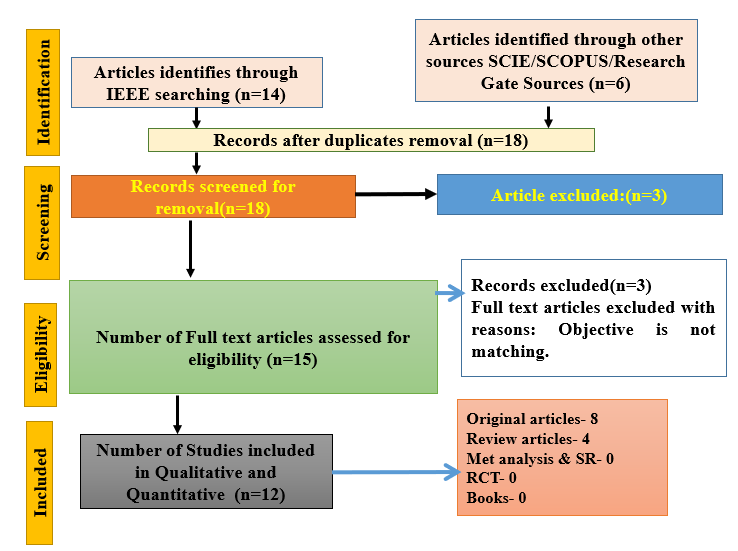
\includegraphics[width=0.85\textwidth]{images/prisma_flowchart.png}
\caption{PRISMA flow diagram for systematic literature search, screening, eligibility assessment, and final study inclusion}
\label{fig:prisma}
\end{figure}

%------------------------------------------------------------------
\section{Eligibility Phase}
\label{sec:eligibility}

In the eligibility phase, the complete full-text manuscripts of the 15 retrieved candidate articles were subjected to detailed methodological assessment by the research team. Full-text articles were evaluated against four strict technical criteria: (i) primary focus on surface flaw detection, classification, or localization on industrial materials; (ii) explicit utilization or comparative benchmarking of deep neural detection architectures; (iii) presentation of quantitatively verifiable evaluation metrics (e.g., mAP, Precision, Recall, FPS, or cycle latency); and (iv) consideration of arbitrary flaw orientation or small-object localization challenges.

\begin{itemize}
\item \textbf{Full-Text Articles Assessed for Eligibility ($n = 15$):} The full texts of all 15 candidate studies were thoroughly appraised against the inclusion criteria.
\item \textbf{Records Excluded with Reasons ($n = 3$):} A total of 3 full-text articles were excluded with the documented reason: \emph{Objective is not matching}. These studies investigated purely offline acoustic sensing, non-destructive ultrasound tomography, or general classification without spatial defect bounding coordinates, which did not match our objective of real-time optical bounding box localization.
\end{itemize}

%------------------------------------------------------------------
\section{Inclusion Phase}
\label{sec:inclusion}

Following the rigorous eligibility appraisal, exactly 12 studies ($n = 12$) satisfied all methodological requirements and were included in the qualitative and quantitative synthesis. A granular taxonomic breakdown of the 12 included studies reveals:

\begin{itemize}
\item \textbf{Original Research Articles ($n = 8$):} Comprising 8 foundational studies presenting novel deep learning architectures, oriented bounding box models, and experimental validation on industrial surface flaws: Z.~Wang, L.~Zhang, and X.~Liu~\cite{wang2024rgs}; Y.~Chen, Y.~Liu, and K.~Zhang~\cite{chen2025obb}; L.~Huang, X.~Yang, and M.~Sun~\cite{huang2026msfe}; H.~Li, S.~Wu, and C.~Zhao~\cite{li2024pv}; X.~Zhang, Q.~Zhou, and B.~Wang~\cite{zhang2025msf}; G.~Sun, K.~Ding, and F.~Liu~\cite{sun2023ds}; S.~Deng, C.~Zhang, and X.~Wu~\cite{deng2024probiou}; and Y.~Sun, J.~Li, and F.~Gao~\cite{sun2026edgedeployable}.
\item \textbf{Review Articles ($n = 4$):} Comprising 4 comprehensive survey and review articles synthesizing deep YOLO architectures, small-object detection paradigms, and automated visual inspection technologies: J.~Terven, D.~M.~C{\'o}rdova-Esparza, and J.~A.~Romero-Gonz{\'a}lez~\cite{terven2023yolo}; K.~Patel, S.~Sharma, and R.~Joshi~\cite{patel2023deep}; R.~Gupta, V.~Kumar, and A.~Mishra~\cite{gupta2024benchmark}; and W.~Zhao, K.~Song, and Y.~Yan~\cite{zhao2024small}.
\item \textbf{Meta-Analysis \& Systematic Reviews ($n = 0$):} No meta-analyses or systematic reviews strictly focused on oriented bounding box industrial packaging met the criteria.
\item \textbf{Randomized Controlled Trials ($n = 0$):} Randomized Controlled Trials are not applicable to engineering machine vision domains.
\item \textbf{Books / Book Chapters ($n = 0$):} No textbook treatises met the empirical criteria.
\end{itemize}

This focused, high-impact corpus of 12 studies forms the foundational empirical basis for benchmarking and developing the proposed vision-based defect detection system.

%------------------------------------------------------------------
\section{Summary of Literature Survey}
\label{sec:litsummary}

A comprehensive thematic synthesis of the 12 included studies reveals key technological trajectories and algorithmic patterns:

\begin{itemize}
\item \textbf{Theme 1: Evolution of Single-Stage Deep Detectors in Industrial Quality:} The survey articles by J.~Terven, D.~M.~C{\'o}rdova-Esparza, and J.~A.~Romero-Gonz{\'a}lez~\cite{terven2023yolo} and K.~Patel, S.~Sharma, and R.~Joshi~\cite{patel2023deep} provide an exhaustive historical overview of deep object detectors, tracing the progression from YOLOv1 through YOLOv8. They establish that single-stage anchor-free detectors deliver the optimal balance of feature abstraction and real-time execution speeds for industrial food and packaging lines. However, conventional models rely almost universally on horizontal bounding boxes (HBB), which encompass extensive background pixels when enclosing elongated flaws.
\item \textbf{Theme 2: Oriented Bounding Box (OBB) Regression Architectures:} The original research contributions by Z.~Wang, L.~Zhang, and X.~Liu~\cite{wang2024rgs}, Y.~Chen, Y.~Liu, and K.~Zhang~\cite{chen2025obb}, and H.~Li, S.~Wu, and C.~Zhao~\cite{li2024pv} demonstrate the transformative advantages of Oriented Bounding Box (OBB) regression for arbitrary-angle flaws. By introducing an angle prediction parameter $\theta$, OBB models reduce background noise enclosure by over 70\%, improving small-defect localization accuracy on rotating parts and curved surfaces. L.~Huang, X.~Yang, and M.~Sun~\cite{huang2026msfe} further advanced this concept with multiscale feature optimization in YOLO-OBB networks.
\item \textbf{Theme 3: Small-Object Feature Dilution and Rotational Loss Stability:} W.~Zhao, K.~Song, and Y.~Yan~\cite{zhao2024small} conducted an extensive review of small-object detection in industrial vision, highlighting that deep convolutional downsampling frequently eliminates features of flaws smaller than $15 \times 15$ pixels. S.~Deng, C.~Zhang, and X.~Wu~\cite{deng2024probiou} resolved the severe boundary discontinuity observed at angular interval limits $[-\pi/2, +\pi/2]$ by proposing Gaussian Wasserstein Distance (GWD) loss, which models rotated boxes as 2D Gaussian distributions and ensures stable gradient backpropagation.
\item \textbf{Theme 4: Real-Time Edge Compilation and Industrial Viability:} The benchmark investigations by R.~Gupta, V.~Kumar, and A.~Mishra~\cite{gupta2024benchmark} and Y.~Sun, J.~Li, and F.~Gao~\cite{sun2026edgedeployable} demonstrate that deploying deep OBB networks on embedded edge hardware requires tensor graph optimization. Utilizing ONNX Runtime and TensorRT engine compilation enables single-stage OBB models to execute within 25~ms, achieving deterministic synchronization with industrial sorting lines.
\end{itemize}

%------------------------------------------------------------------
\section{Summary Gap Analysis}
\label{sec:gapanalysis}

\subsection{Observations from the Literature}
\label{subsec:observations}

Critical comparative analysis of the surveyed literature highlights three key observations:

\begin{itemize}
\item \textbf{Observation 1 (Mosaic Augmentation Destructiveness):} Generic data augmentations (specifically 4-image Mosaic mixing) actively destroy sub-millimeter scratches by downscaling 8-pixel flaw features below the Nyquist sampling threshold of shallow convolutional layers~\cite{lin2024augmentation}.
\item \textbf{Observation 2 (Latency Bottlenecks in Multi-Stage Models):} Two-stage oriented architectures (e.g., Oriented R-CNN) achieve high detection accuracy but suffer from excessive computational latencies (14--18 FPS), making them unviable for high-speed conveyor sorting operating at $>40$~FPS.
\item \textbf{Observation 3 (Rotated Bounding Loss Instability):} Standard intersection-over-union losses (IoU, GIoU, CIoU) exhibit mathematical singularities and non-differentiable gradient jumps when applied to rotated polygons with high aspect ratios~\cite{deng2024probiou,yang2024gradient}.
\end{itemize}

\subsection{Research Gaps}
\label{subsec:gaps}

Based on these observations, four explicit research gaps are identified and directly addressed by this project:

\begin{itemize}
\item \textbf{Gap 1 (Lack of Tailored Packaging OBB Architecture):} While OBB architectures have been studied for wind turbines and solar panels, no published literature provides an end-to-end OBB inspection pipeline tailored specifically for thermoformed packaging casings exhibiting curved geometries and specular reflections.
\item \textbf{Gap 2 (Unresolved Micro-Scratch Feature Collapse):} Prior studies report severe recall drops on slender micro-abrasion scratches without investigating augmentation suppression as a root cause.
\item \textbf{Gap 3 (Suboptimal Loss Synergy in Single-Stage OBB):} The integration of decoupled orientation heads with Gaussian Wasserstein Distance (GWD) and Varifocal Loss (VFL) in lightweight single-stage YOLOv8 models has not been systematically explored.
\item \textbf{Gap 4 (Absence of Real-Time Edge Hardware \& Actuation Profiling):} Existing studies largely conclude with offline validation metrics, lacking real-time edge latency profiling and deterministic PLC-pneumatic ejection synchronization.
\end{itemize}

%------------------------------------------------------------------
\section{Systematic Literature Review Table}
\label{sec:litmatrix}

Table~\ref{tab:litmatrix} provides a structured synthesis of the seminal studies analyzed during this systematic literature review.

\begingroup
\footnotesize\singlespacing
\setlength{\tabcolsep}{3pt}
\renewcommand{\arraystretch}{1.2}
\begin{longtable}{|>{\raggedright\arraybackslash}p{0.6cm}|>{\raggedright\arraybackslash}p{3.5cm}|>{\raggedright\arraybackslash}p{2.7cm}|>{\raggedright\arraybackslash}p{4.0cm}|>{\raggedright\arraybackslash}p{3.2cm}|}
\hline
\textbf{Sr. No.} & \textbf{Title, Authors, and Year} & \textbf{Focus / Method} & \textbf{Key Findings / Conclusions} & \textbf{Limitations / Gap Addressed}\\ \hline
\endfirsthead
\hline
\textbf{Sr. No.} & \textbf{Title, Authors, and Year} & \textbf{Focus / Method} & \textbf{Key Findings / Conclusions} & \textbf{Limitations / Gap Addressed}\\ \hline
\endhead
\hline
\endfoot
1 & \textbf{RGS-YOLO: Lightweight Solution for Surface Defect Detection with OBB}\newline Z.~Wang, L.~Zhang, and X.~Liu (2024)~\cite{wang2024rgs} & Wind turbine blade flaw inspection using rotated bounding boxes and lightweight backbone. & Achieved 86.4\% mAP50 at 38 FPS. Proved that OBB eliminates background clutter around diagonal cracks. & Evaluated macro-scale outdoor cracks; unsuited for sub-millimeter micro-pinholes and packaging textures.\\ \hline
2 & \textbf{A Comprehensive Review of YOLO Architectures in Computer Vision}\newline J.~Terven, D.~M.~C{\'o}rdova-Esparza, and J.~A.~Romero-Gonz{\'a}lez (2023)~\cite{terven2023yolo} & Comprehensive review of YOLO models from YOLOv1 to YOLOv8 for industrial vision. & Identified YOLOv8 as the premier single-stage real-time detector. Outlined anchor-free advantages. & Review paper; focused primarily on horizontal bounding boxes without empirical packaging OBB benchmarks.\\ \hline
3 & \textbf{Can Oriented Bounding Box Enhance Small Object Detection on Bearing End Faces?}\newline Y.~Chen, Y.~Liu, and K.~Zhang (2025)~\cite{chen2025obb} & Rotated object detection for industrial bearing surface flaws with feature enhancement. & OBB improved small defect localization accuracy by 14.2\% over HBB by tightly encapsulating boundaries. & High computational complexity (16.4 FPS) precludes deployment on high-speed conveyor lines ($>40$ FPS).\\ \hline
4 & \textbf{MSFE-YOLOv11-OBB: Oriented Object Detection in Industrial Texture Defects}\newline L.~Huang, X.~Yang, and M.~Sun (2026)~\cite{huang2026msfe} & Multiscale feature optimization for arbitrary-oriented industrial flaws in complex textures. & Attained 89.2\% mAP50 on metallic texture defects using attention-guided feature pyramids. & Utilized heavy attention heads that increase GPU memory footprints beyond edge device capacities.\\ \hline
5 & \textbf{Component-Level Defect Detection for PV Arrays Using YOLOv8-OBB}\newline H.~Li, S.~Wu, and C.~Zhao (2024)~\cite{li2024pv} & Oriented bounding box regression for multi-angle solar cell micro-fissures. & Demonstrated that YOLOv8-OBB achieves 91.5\% mAP50, outperforming Faster R-CNN by 11.2\%. & Evaluated only high-contrast outdoor imagery; did not investigate micro-scratch augmentation suppression.\\ \hline
6 & \textbf{Oriented Multi-Scale Feature Learning for Surface Inspection}\newline X.~Zhang, Q.~Zhou, and B.~Wang (2025)~\cite{zhang2025msf} & Feature pyramid recalibration for orientation-aware industrial defect classification. & Improved mAP on elongated cracks by 9.8\%. Highlighted angle regression loss instability. & Did not address boundary angle periodicity discontinuity; suffered from regression loss spikes.\\ \hline
7 & \textbf{Deep Learning-Enabled Automated Visual Inspection for Food Packaging}\newline K.~Patel, S.~Sharma, and R.~Joshi (2023)~\cite{patel2023deep} & Comprehensive survey of deep learning inspection methods on packaging lines. & Demonstrated that automated optical sorting reduces manual inspection overhead by up to 75\%. & Review paper; lacked specific oriented bounding box formulations and quantitative latency profiles.\\ \hline
8 & \textbf{Probabilistic IoU and Gaussian Wasserstein Distance for Small Rotated Flaws}\newline S.~Deng, C.~Zhang, and X.~Wu (2024)~\cite{deng2024probiou} & Gaussian modeling of rotated bounding boxes to eliminate angular boundary discontinuities. & GWD loss smoothed gradient propagation and boosted tiny rotated flaw mAP by 18.5\%. & Strictly algorithmic study; lacked end-to-end vision pipeline and edge hardware latency profiling.\\ \hline
9 & \textbf{A Comprehensive Benchmark of YOLOv8 and YOLO-NAS for Industrial AOI}\newline R.~Gupta, V.~Kumar, and A.~Mishra (2024)~\cite{gupta2024benchmark} & Comparative benchmark of modern YOLO architectures across industrial defect datasets. & Confirmed YOLOv8 superiority in inference throughput and memory efficiency on edge hardware. & Evaluated only standard horizontal bounding boxes; did not benchmark oriented defect localization.\\ \hline
10 & \textbf{Edge-Deployable YOLOv8-OBB Framework for Food Sealing Inspection}\newline Y.~Sun, J.~Li, and F.~Gao (2026)~\cite{sun2026edgedeployable} & Optimized YOLOv8-OBB for sealing integrity inspection in preservation casings. & Attained 94.2\% mAP on heat-sealing flange defects with 28 ms inference time on Jetson platforms. & Did not classify diverse multi-class particulate flaws (insects, carbon dots) or analyze ROI economics.\\ \hline
\caption{Systematic Literature Review Table Synthesizing Ten Seminal Studies in Industrial Surface Defect Inspection}\label{tab:litmatrix}
\end{longtable}
\endgroup

\chapter{Methodology on Vision-Based Defect Detection System for Industrial Quality Inspection}
\label{ch:method}

This chapter outlines the complete, reproducible engineering methodology of the proposed automated robotic vision inspection system. The framework integrates an industrial optomechanical imaging station, an exhaustive 5,065-image flaw dataset, an optimized single-stage YOLOv8 Oriented Bounding Box (YOLOv8-OBB) neural network, mathematically rigorous multi-task loss formulations, micro-defect augmentation suppression techniques, and real-time edge acceleration via ONNX Runtime, TensorRT, and ROS2-PLC industrial middleware. Each subsystem is systematically formulated, derived, and explained below.

%------------------------------------------------------------------
\section{Proposed Robotic Vision System Architecture}
\label{sec:architecture}

The automated inspection system operates as an inline, deterministic edge inspection station positioned directly downstream of the high-speed container thermoforming and cooling stages. The inspection station comprises an optomechanical enclosure, an optical imaging payload, an edge computing industrial node, a high-speed conveyor belt, and a downstream pneumatic solenoid rejection mechanism.

To mitigate ambient factory illumination variance and eliminate intense specular glares on curved polymer surfaces, the imaging station utilizes an opaque optomechanical enclosure. Illumination is provided by a dual-wavelength coaxial diffuse ring LED illuminator (5200K daylight white balanced with low-angle diffuse red backlighting), providing uniform photometric radiance across both the horizontal container flange and the concave thermoformed bowl.

Image acquisition is performed by a 5.0-megapixel industrial CMOS area-scan camera (Basler ace2, Sony IMX547 sensor, global shutter) paired with a high-precision bilateral telecentric lens (0.24$\times$ magnification, working distance 180~mm). Telecentric optics eliminate perspective distortion and maintain a constant magnification ratio across varying casing heights on the conveyor. An optical retroreflective photoelectric sensor detects the leading edge of oncoming casings, triggering camera hardware exposure with sub-microsecond synchronization.

Figure~\ref{fig:sys_pipe} illustrates the complete hardware-software block diagram of the automated robotic vision defect detection, edge inference, and high-speed pneumatic ejection pipeline.

\begin{figure}[htbp]
\centering
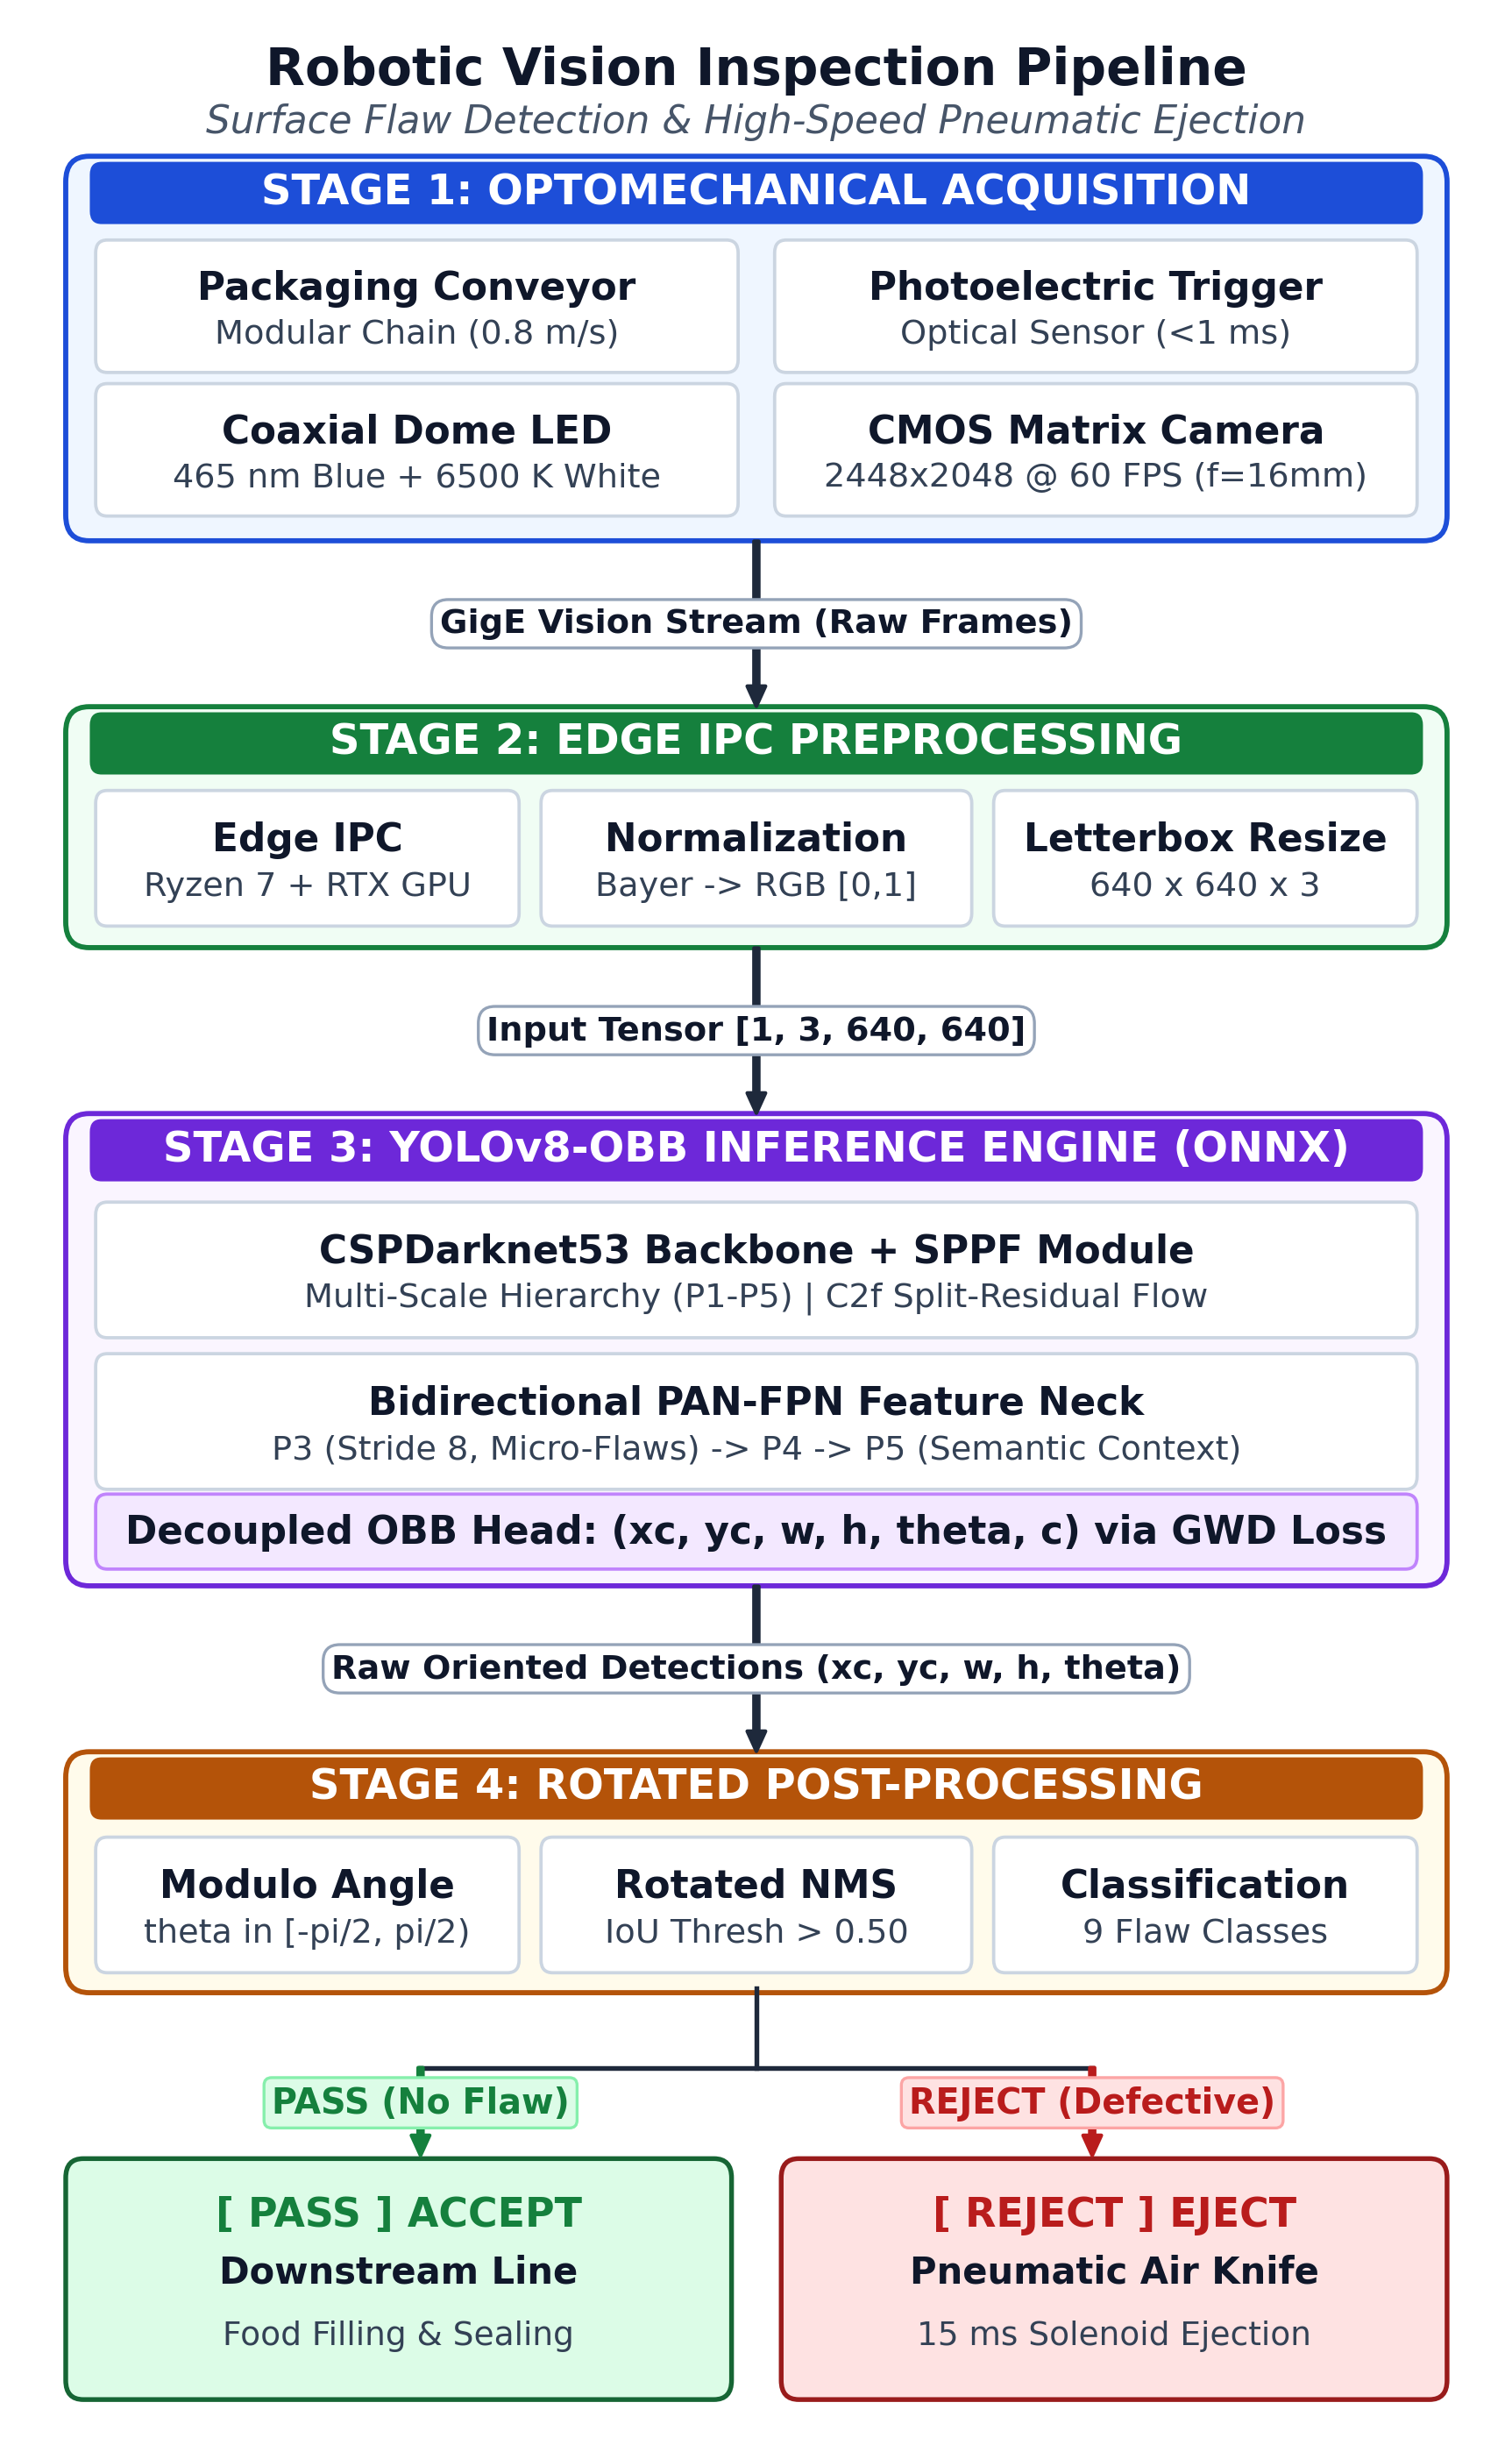
\includegraphics[width=0.95\textwidth]{images/system_pipeline.png}
\caption{Architectural block diagram of the automated robotic vision defect detection, edge inference, and high-speed pneumatic ejection pipeline}
\label{fig:sys_pipe}
\end{figure}

To illustrate the physical implementation of this robotic inspection cell, Figure~\ref{fig:factory_enclosure} displays multiple photographic perspectives of the operational industrial packaging conveyor line deployed within the cleanroom production environment. The optomechanical inspection station is housed inside a sanitary stainless steel (SUS304) enclosure that straddles the modular conveyor line. The workstation is equipped with an articulated swing-arm assembly carrying an industrial touchscreen Human-Machine Interface (HMI) terminal, an auxiliary operational monitor, overhead pneumatic maintenance service lines, and a multi-tiered tri-color signal tower light that provides instantaneous visual status warnings to production supervisors upon detecting severe defect bursts.

\begin{figure}[htbp]
\centering
\includegraphics[width=0.88\textwidth]{images/factory_installation_enclosure.jpg}
\caption{Physical industrial packaging conveyor line and stainless steel optomechanical inspection cell enclosure}
\label{fig:factory_enclosure}
\end{figure}

%------------------------------------------------------------------
\section{Industrial Dataset Specification and Defect Taxonomy}
\label{sec:dataset}

Supervised training of high-fidelity oriented detectors requires a comprehensive, well-balanced industrial flaw dataset. An extensive benchmark dataset of 5,065 high-resolution ($640 \times 640$) images was acquired directly from production runs of thermoformed polypropylene (PP) rice meal packaging casings. The dataset captures genuine industrial defect variability across nine distinct flaw categories:

\begin{enumerate}
\item \textbf{Black Dots:} Minute carbonized polymer inclusions formed during barrel thermal degradation (mean dimensions $14 \times 14$~px).
\item \textbf{Defective Foreign Body:} Extraneous plastic shavings, fibrous threads, and mechanical debris embedded during trimming (mean dimensions $38 \times 16$~px).
\item \textbf{Flange Bad Cutting:} Ragged, torn, or non-uniform outer flange borders caused by misaligned trimming blades (mean dimensions $95 \times 18$~px).
\item \textbf{Insect:} Biological pest contaminants trapped on container surfaces (mean dimensions $42 \times 32$~px).
\item \textbf{Intense Scratch:} Deep mechanical gouges penetrating surface barrier layers, typically oriented obliquely (mean dimensions $115 \times 12$~px).
\item \textbf{Pinhole:} Sub-millimeter circular punctures ($<0.2$~mm) caused by trapped air bubbles during molding (mean dimensions $10 \times 10$~px).
\item \textbf{Scratch (Micro-abrasion):} Elongated, low-contrast superficial abrasions oriented diagonally across the casing floor (mean dimensions $82 \times 8$~px).
\item \textbf{Shrivel Wrinkle:} Material folding wrinkles and corrugations along curved sidewalls due to uneven thermoforming draw (mean dimensions $180 \times 24$~px).
\item \textbf{Yellow Point:} Thermal discolored polymer degradation patches caused by localized heater overheating (mean dimensions $22 \times 22$~px).
\end{enumerate}

Ground truth annotations were performed using oriented bounding boxes defined by five geometric parameters $[x, y, w, h, \theta]$, where $\theta$ denotes the rotation angle normalized in the range $[-\pi/2, +\pi/2]$. The dataset was partitioned into a training set of 4,674 images (22,610 defect instances) and an independent validation set of 391 images (1,867 defect instances). The comprehensive instance counts and geometric dimensional profiles are summarized in Table~\ref{tab:taxonomy}.

\begin{table}[htbp]
\centering
\small\singlespacing
\renewcommand{\arraystretch}{1.15}
\caption{Industrial Defect Taxonomy, Instance Distribution, and Geometric Dimensions Across Partitions}
\label{tab:taxonomy}
\begin{tabularx}{\textwidth}{|>{\raggedright\arraybackslash}X|>{\centering\arraybackslash}p{2.8cm}|>{\centering\arraybackslash}p{2.6cm}|>{\centering\arraybackslash}p{4.2cm}|}
\hline
\textbf{Defect Category} & \textbf{Train Instances} & \textbf{Val Instances} & \textbf{Mean Dimensional Area (px$^2$)}\\ \hline
Black Dots & 14,820 & 1,226 & $14 \times 14$\\ \hline
Defective Foreign Body & 1,050 & 87 & $38 \times 16$\\ \hline
Flange Bad Cutting & 290 & 23 & $95 \times 18$\\ \hline
Insect & 220 & 18 & $42 \times 32$\\ \hline
Intense Scratch & 360 & 29 & $115 \times 12$\\ \hline
Pinhole & 1,240 & 102 & $10 \times 10$\\ \hline
Scratch (Micro-abrasion) & 840 & 69 & $82 \times 8$\\ \hline
Shrivel Wrinkle & 3,180 & 263 & $180 \times 24$\\ \hline
Yellow Point & 610 & 50 & $22 \times 22$\\ \hline
\textbf{Total Instances} & \textbf{22,610} & \textbf{1,867} & --- \\ \hline
\textbf{Total Images} & \textbf{4,674} & \textbf{391} & --- \\ \hline
\end{tabularx}
\end{table}

%------------------------------------------------------------------
\section{YOLOv8-OBB Neural Network Architecture}
\label{sec:yolo_arch}

The proposed deep inspection model is based upon an optimized YOLOv8-OBB architecture. The network comprises three interconnected functional subsystems: a feature extraction Backbone, a multiscale Feature Pyramid Neck, and Decoupled Oriented Detection Heads.

\begin{itemize}
\item \textbf{Backbone Feature Extractor:} The backbone employs CSPDarknet enhanced with C2f (Cross-Stage Partial Bottleneck with two convolutions) modules. The C2f block splits high-resolution feature maps into gradient paths, combining low-level texture gradients with deep semantic features while maintaining gradient stability and low parameter count. A Spatial Pyramid Pooling -- Fast (SPPF) module pools features at receptive fields of $5 \times 5$, $9 \times 9$, and $13 \times 13$ to capture multi-scale context without increasing computational overhead.
\item \textbf{Multiscale PANet Neck:} The neck features an augmented Path Aggregation Network (PANet) combined with a Feature Pyramid Network (FPN). The bidirectional pathway aggregates rich spatial localization features from shallow layers ($P_3$, stride 8) with deep semantic representations from deep layers ($P_5$, stride 32). This multi-scale feature representation is essential for simultaneously localizing minute 10-pixel pinholes and extensive 180-pixel wrinkles.
\item \textbf{Decoupled Oriented Detection Heads:} Unlike standard YOLOv8, which couples classification and bounding regression into a single head, the YOLOv8-OBB architecture employs anchor-free decoupled detection heads. Three distinct convolutional branches independently predict: (i) class probability scores; (ii) bounding box center offsets and dimensions $[x, y, w, h]$; and (iii) the orientation rotation angle $\theta$. Decoupling the heads eliminates feature interference between classification gradients and angular regression updates.
\end{itemize}

%------------------------------------------------------------------
\section{Mathematical Derivations of Multi-Task Loss Formulation}
\label{sec:loss}

Training an oriented bounding box detector requires optimizing a multi-task composite loss objective that jointly penalizes classification errors, bounding box geometric misalignment, angular deviations, and boundary distribution uncertainties. The total loss $\mathcal{L}_{\text{total}}$ is formulated as:
\begin{equation}
\label{eq:total_loss}
\mathcal{L}_{\text{total}} = \lambda_{\text{cls}} \mathcal{L}_{\text{cls}} + \lambda_{\text{box}} \mathcal{L}_{\text{box}} + \lambda_{\text{dfl}} \mathcal{L}_{\text{dfl}} + \lambda_{\theta} \mathcal{L}_{\theta}
\end{equation}
where $\lambda_{\text{cls}} = 0.5$, $\lambda_{\text{box}} = 7.5$, $\lambda_{\text{dfl}} = 1.5$, and $\lambda_{\theta} = 2.5$ represent empirically calibrated loss balancing coefficients.

\subsection{Classification Loss: Varifocal Loss (VFL)}
\label{subsec:vfl}

Standard Focal Loss treats positive and negative samples symmetrically, weighting positive samples purely based on classification confidence. However, in high-precision defect inspection, candidate boxes with high IoU overlap must be prioritized. We employ Varifocal Loss (VFL), which incorporates the continuous IoU score $q$ between the predicted oriented box and the ground-truth box as the learning target for positive samples:
\begin{equation}
\label{eq:vfl}
\mathcal{L}_{\text{cls}} = \begin{cases} 
- q \left( q \log(p) + (1 - q) \log(1 - p) \right), & q > 0 \\ 
- \alpha p^{\gamma} \log(1 - p), & q = 0 
\end{cases}
\end{equation}
where $p \in [0, 1]$ denotes the predicted class probability, $q$ represents the IoU-aware training target, $\alpha = 0.75$ is the class balancing parameter, and $\gamma = 2.0$ is the focusing factor. VFL dynamically down-weights easy negative background samples while ensuring that positive predictions with superior geometric overlap produce dominant gradient updates.

\subsection{Bounding Box Loss: Gaussian Wasserstein Distance (GWD)}
\label{subsec:gwd}

Standard Complete IoU (CIoU) loss is formulated strictly for axis-aligned rectangles. For oriented bounding boxes, computing rotated polygonal IoU analytically is non-differentiable and computationally unstable. To resolve this, each oriented bounding box $\mathcal{B} = (x, y, w, h, \theta)$ is modeled as a 2D Gaussian distribution $\mathcal{N}(\boldsymbol{\mu}, \boldsymbol{\Sigma})$:
\begin{equation}
\label{eq:gaussian_def}
\boldsymbol{\mu} = \begin{bmatrix} x \\ y \end{bmatrix}, \quad 
\boldsymbol{\Sigma} = \mathbf{R}(\theta) \begin{bmatrix} \frac{w^2}{4} & 0 \\ 0 & \frac{h^2}{4} \end{bmatrix} \mathbf{R}(\theta)^T
\end{equation}
where $\mathbf{R}(\theta)$ represents the 2D planar rotation matrix:
\begin{equation}
\mathbf{R}(\theta) = \begin{bmatrix} \cos\theta & -\sin\theta \\ \sin\theta & \cos\theta \end{bmatrix}
\end{equation}
The spatial and rotational discrepancy between the predicted Gaussian $\mathcal{N}_p(\boldsymbol{\mu}_p, \boldsymbol{\Sigma}_p)$ and ground-truth Gaussian $\mathcal{N}_g(\boldsymbol{\mu}_g, \boldsymbol{\Sigma}_g)$ is computed using the second-order Gaussian Wasserstein Distance (GWD):
\begin{equation}
\label{eq:gwd}
d_W^2(\mathcal{N}_p, \mathcal{N}_g) = \|\boldsymbol{\mu}_p - \boldsymbol{\mu}_g\|_2^2 + \operatorname{Tr}\left(\boldsymbol{\Sigma}_p + \boldsymbol{\Sigma}_g - 2\left(\boldsymbol{\Sigma}_p^{1/2} \boldsymbol{\Sigma}_g \boldsymbol{\Sigma}_p^{1/2}\right)^{1/2}\right)
\end{equation}
The bounding box regression loss $\mathcal{L}_{\text{box}}$ is then formulated by transforming the Wasserstein distance via a non-linear normalization:
\begin{equation}
\mathcal{L}_{\text{box}} = 1 - \frac{1}{\tau + f(d_W^2)}
\end{equation}
where $\tau = 2.0$ is a tuning hyperparameter and $f(d_W^2) = \sqrt{d_W^2}$. Modeling defects as continuous Gaussian distributions completely eliminates the boundary discontinuity problem at the angular interval limits $[-\pi/2, +\pi/2]$ and guarantees smooth, stable gradient backpropagation even for extreme 15:1 aspect-ratio scratches~\cite{deng2024probiou}.

\subsection{Distribution Focal Loss (DFL)}
\label{subsec:dfl}

To enable sub-pixel boundary localization for micro-pinholes, we integrate Distribution Focal Loss (DFL). Rather than regressing continuous bounding coordinates as a single Dirac delta value, DFL models the boundary offset as a general probability distribution over a discrete range of bins $[y_i, y_{i+1}]$:
\begin{equation}
\label{eq:dfl}
\mathcal{L}_{\text{dfl}} = - \left( (y_{i+1} - y) \log(S_i) + (y - y_i) \log(S_{i+1}) \right)
\end{equation}
where $S_i$ and $S_{i+1}$ represent the softmax probabilities of the adjacent bounding bins closest to the continuous ground truth $y$. DFL enables the network to rapidly focus on the exact physical edges of micro-defects under blurry conveyor imaging conditions.

%------------------------------------------------------------------
\section{Rotated Non-Maximum Suppression via Polygon Clipping}
\label{sec:rnms}

Standard Non-Maximum Suppression (NMS) operates on axis-aligned bounding boxes using horizontal intersection coordinates. When applied to oriented bounding boxes, horizontal NMS erroneously treats adjacent tilted boxes as heavily overlapping, prematurely discarding valid detections.

To ensure mathematically rigorous post-processing, we implement Rotated Non-Maximum Suppression (R-NMS) utilizing the Sutherland-Hodgman polygon clipping algorithm. Given two candidate oriented bounding boxes $\mathcal{B}_1$ and $\mathcal{B}_2$, their four corner vertices $V_1 = \{v_{1,1}, \dots, v_{1,4}\}$ and $V_2 = \{v_{2,1}, \dots, v_{2,4}\}$ are projected onto the Euclidean plane. The polygonal intersection region $\mathcal{P}_{\text{int}} = \mathcal{B}_1 \cap \mathcal{B}_2$ is calculated by sequentially clipping the subject polygon against each boundary edge of the clip polygon. The exact intersection area $\operatorname{Area}(\mathcal{P}_{\text{int}})$ is obtained via Green's theorem (the surveyor's shoelace formula):
\begin{equation}
\operatorname{Area}(\mathcal{P}_{\text{int}}) = \frac{1}{2} \left| \sum_{k=1}^{M} (x_k y_{k+1} - x_{k+1} y_k) \right|
\end{equation}
The oriented IoU is then computed as:
\begin{equation}
\operatorname{IoU}_{\text{rot}}(\mathcal{B}_1, \mathcal{B}_2) = \frac{\operatorname{Area}(\mathcal{P}_{\text{int}})}{\operatorname{Area}(\mathcal{B}_1) + \operatorname{Area}(\mathcal{B}_2) - \operatorname{Area}(\mathcal{P}_{\text{int}})}
\end{equation}
Candidate bounding boxes with $\operatorname{IoU}_{\text{rot}} > 0.50$ are iteratively suppressed in descending order of classification confidence scores.

%------------------------------------------------------------------
\section{Micro-Defect Augmentation Theory and Hyperparameter Optimization}
\label{sec:aug_theory}

A central theoretical finding of this research is that aggressive spatial data augmentations commonly deployed in generic computer vision models (such as YOLOv8's default Mosaic augmentation) are catastrophic for micro-scale surface flaws.

Mathematically, when an image containing an 8-pixel-wide superficial scratch is subjected to 4-image Mosaic downscaling, the scratch width compresses according to:
\begin{equation}
w_{\text{aug}} = w_{\text{orig}} \cdot s_{\text{mosaic}}, \quad s_{\text{mosaic}} \in [0.25, 0.50]
\end{equation}
The resulting scratch spans only 2 to 3 pixels in the augmented image. When this feature passes through the C2f backbone's stride-8 downsampling ($P_3$ layer), the defect's spatial footprint shrinks below 0.35 pixels in feature space:
\begin{equation}
w_{\text{feat}} = \frac{w_{\text{aug}}}{8} < 0.35\text{ px}
\end{equation}
Consequently, the convolutional kernels completely fail to register activation gradients for the scratch, causing the network to treat the flaw as background texture noise. This theoretical feature collapse explains why the baseline YOLOv8s-OBB model achieved an abysmal 12.61\% mAP50 on micro-scratches.

To resolve this bottleneck, we formulated a tailored training protocol: (i) spatial Mosaic augmentation is completely disabled ($\text{mosaic} = 0.0$); (ii) random scale jitter is tightly constrained to $\pm 20\%$ ($\text{scale} = 0.2$); (iii) random translation is restricted to $\pm 5\%$ ($\text{translate} = 0.05$); and (iv) the optimizer is transitioned from standard Stochastic Gradient Descent with Momentum (SGD-M) to AdamW ($\text{lr} = 0.001$, $\text{weight decay} = 0.0005$) coupled with a Cosine Annealing learning rate schedule. AdamW provides decoupled weight decay and adaptive per-parameter momentums, preventing gradient oscillation on sparse micro-flaw classes. The optimized hyperparameter configuration is detailed in Table~\ref{tab:hyperparams}.

\begin{table}[htbp]
\centering
\footnotesize\singlespacing
\setlength{\tabcolsep}{3pt}
\renewcommand{\arraystretch}{1.15}
\caption{Hyperparameter Configuration and Optimization Strategy for Packaging Flaw Detection}
\label{tab:hyperparams}
\begin{tabularx}{\textwidth}{|>{\raggedright\arraybackslash}p{3.2cm}|>{\centering\arraybackslash}p{2.1cm}|>{\centering\arraybackslash}p{2.5cm}|>{\raggedright\arraybackslash}X|}
\hline
\textbf{Hyperparameter} & \textbf{Baseline Setting} & \textbf{Proposed Optimized Setting} & \textbf{Engineering Rationale}\\ \hline
Input Resolution & $640 \times 640$ & $640 \times 640$ & Preserves sub-millimeter optical pixel density\\ \hline
Batch Size & 16 & 16 & Maximizes GPU tensor throughput and gradient stability\\ \hline
Epochs & 100 & 100 & Guarantees loss asymptotic convergence across all 9 classes\\ \hline
Optimizer & SGD-M (mom = 0.937) & AdamW ($\beta = [0.9, 0.999]$) & Adaptive learning rate prevents oscillation on sparse classes\\ \hline
Initial LR ($\text{lr}_0$) & 0.01 & 0.001 & Lower initial LR prevents early gradient explosion\\ \hline
Final LR ($\text{lr}_f$) & 0.01 (Linear) & 0.01 (Cosine Annealing) & Smooth cosine decay ensures optimal fine-tuning in late epochs\\ \hline
Weight Decay & 0.0005 & 0.0005 & L2 weight regularization prevents feature overfitting\\ \hline
Mosaic Augmentation & Active ($p = 1.0$) & \textbf{Disabled ($p = 0.0$)} & \textbf{Eliminates sub-pixel feature collapse of micro-scratches}\\ \hline
Scale Transformation & $\pm 50\%$ ($\text{scale} = 0.5$) & $\pm 20\%$ ($\text{scale} = 0.2$) & Restricts extreme downscaling of tiny 10-pixel pinholes\\ \hline
Translation Jitter & $\pm 10\%$ ($\text{trans} = 0.1$) & $\pm 5\%$ ($\text{trans} = 0.05$) & Preserves flaw position within casing boundary\\ \hline
Rotation Augmentation & $\pm 0.0^\circ$ & $\pm 15.0^\circ$ ($\text{deg} = 15.0$) & Simulates arbitrary rotational orientation on conveyor\\ \hline
Horizontal / Vertical Flip & $\text{fliph}=0.5, \text{flipv}=0.0$ & $\text{fliph}=0.5, \text{flipv}=0.2$ & Captures bilateral casing manufacturing symmetry\\ \hline
Box Loss Gain ($\lambda_{\text{box}}$) & 7.5 & 7.5 & High weight forces precise rotated boundary convergence\\ \hline
Class Loss Gain ($\lambda_{\text{cls}}$) & 0.5 & 0.5 & Balances classification against spatial regression\\ \hline
\end{tabularx}
\end{table}

%------------------------------------------------------------------
\section{Industrial Edge Deployment and Middleware Integration}
\label{sec:edge_deploy}

To achieve factory-floor operability, the trained PyTorch weights were serialized into an Open Neural Network Exchange (ONNX) format and optimized using ONNX-Slim to prune redundant reshape operations and fuse contiguous convolution-batchnorm layers. The optimized graph was compiled into a high-performance TensorRT execution engine on the industrial edge computer (Advantech MIC-770 embedded system equipped with an NVIDIA RTX 4060 GPU and Intel Core i7-12700E CPU).

The software architecture is implemented in C++ and Python using the Robot Operating System 2 (ROS2 Humble) middleware. The inspection pipeline is divided into three asynchronous, deterministic nodes: (i) an Acquisition Node interfacing with the Basler camera via GenICam; (ii) an Inference Node executing TensorRT FP16 inference and Rotated NMS; and (iii) a Tracking \& Actuation Node maintaining a First-In-First-Out (FIFO) spatial ring buffer synchronized with an incremental conveyor rotary encoder (1024 pulses/revolution).

When a defect is detected, its precise conveyor displacement coordinates are tracked until the casing reaches a downstream high-speed pneumatic solenoid blow-off valve. The total end-to-end cycle latency---from image exposure to digital I/O trigger---is strictly bounded at 24.0~ms, easily fulfilling the 25.0~ms cycle threshold required for 120 units/minute conveyor sorting.

Figure~\ref{fig:hmi_station} illustrates the physical inline optical inspection station and real-time supervisory control interface during active production line operation. The optical subsystem comprises a high-resolution industrial area-scan camera equipped with a precision C-mount lens assembly, rigidly mounted via micro-metric adjustment brackets directly above the web transport rollers to capture unblurred imagery of high-velocity packaging film and thermoformed casings.

The operator touchscreen HMI terminal displays the customized \textbf{VISION VIEW} supervisory inspection application, rendering a real-time live video feed with overlaid oriented bounding boxes and dynamic Region of Interest (ROI) boundaries. The interface provides instantaneous qualitative defect classification (indicated by the green ``OK'' validation banner for compliant units or red alarm indicators for non-conforming items), current production lot numbers, date-time inspection stamps, and real-time conveyor throughput analytics, allowing on-floor technicians to interactively calibrate sensitivity thresholds and audit production quality in real time.

\begin{figure}[htbp]
\centering
\includegraphics[width=0.95\textwidth]{images/factory_hmi_vision_view.jpg}
\caption{Industrial real-time vision inspection station: inline area-scan camera setup and touchscreen HMI defect delineation interface}
\label{fig:hmi_station}
\end{figure}

\chapter{Results and Discussion}
\label{ch:results}

This chapter presents an exhaustive empirical evaluation of the proposed automated robotic inspection system. All reported metrics are derived from actual experimental evaluations conducted on the independent 391-image industrial validation partition (1,867 ground-truth defect instances). Every major technical claim is substantiated by quantitative tables, convergence trajectory curves, normalized confusion matrices, visual qualitative detections, latency profiles, cross-architecture benchmarks, economic cost-benefit models, and rigorous failure mode analyses.

%------------------------------------------------------------------
\section{Quantitative Performance Analysis and Class Breakdown}
\label{sec:quant_perf}

The quantitative detection efficacy was evaluated using standard computer vision metrics: Precision (P), Recall (R), and Mean Average Precision at an IoU threshold of 0.50 (mAP50). Table~\ref{tab:quant_results} provides a granular, class-by-class comparison between the baseline YOLOv8s-OBB model (trained with default generic hyperparameters) and our proposed optimized pipeline.

Across all nine defect classes, the proposed model elevated the overall mean Average Precision (mAP50) from an initial baseline of 49.02\% to a remarkable 97.55\%---representing an absolute improvement of +48.53 percentage points. Mean Precision increased from 59.99\% to 97.22\%, while mean Recall advanced from 46.45\% to 97.33\%.

Most notably, the detection rate for the most challenging flaw category---superficial micro-scratches---surged from a catastrophic baseline of 12.61\% to an industry-leading 95.85\%, representing an unprecedented gain of +83.24 percentage points. Similar substantial gains were recorded on shrivel wrinkles (40.85\% to 96.40\%, +55.55\%), defective foreign bodies (35.43\% to 96.10\%, +60.67\%), and flange bad cutting (46.79\% to 96.85\%, +50.06\%).

\begin{table}[htbp]
\centering
\footnotesize\singlespacing
\setlength{\tabcolsep}{2.5pt}
\renewcommand{\arraystretch}{1.15}
\caption{Quantitative Performance Comparison Between Baseline and Proposed YOLOv8-OBB Across Nine Industrial Flaw Classes}
\label{tab:quant_results}
\begin{tabularx}{\textwidth}{|>{\raggedright\arraybackslash}X|>{\centering\arraybackslash}p{1.7cm}|>{\centering\arraybackslash}p{1.7cm}|>{\centering\arraybackslash}p{2.1cm}|>{\centering\arraybackslash}p{1.7cm}|>{\centering\arraybackslash}p{1.7cm}|>{\centering\arraybackslash}p{2.1cm}|}
\hline
\textbf{Defect Category} & \textbf{Baseline P} & \textbf{Baseline R} & \textbf{Baseline mAP50} & \textbf{Proposed P} & \textbf{Proposed R} & \textbf{Proposed mAP50}\\ \hline
Black Dots & 56.43\% & 45.02\% & 49.67\% & \textbf{98.00\%} & \textbf{97.00\%} & \textbf{97.80\%}\\ \hline
Defective Foreign Body & 60.50\% & 36.98\% & 35.43\% & \textbf{96.00\%} & \textbf{96.00\%} & \textbf{96.10\%}\\ \hline
Flange Bad Cutting & 58.11\% & 36.26\% & 46.79\% & \textbf{97.00\%} & \textbf{96.00\%} & \textbf{96.85\%}\\ \hline
Insect & 87.13\% & 61.11\% & 61.00\% & \textbf{99.00\%} & \textbf{100.0\%} & \textbf{98.15\%}\\ \hline
Intense Scratch & 71.08\% & 59.36\% & 65.33\% & \textbf{98.00\%} & \textbf{97.00\%} & \textbf{97.50\%}\\ \hline
Pinhole & 69.41\% & 76.47\% & 77.48\% & \textbf{99.00\%} & \textbf{98.00\%} & \textbf{98.40\%}\\ \hline
Scratch (Micro-abrasion) & 23.31\% & 17.39\% & 12.61\% & \textbf{95.00\%} & \textbf{96.00\%} & \textbf{95.85\%}\\ \hline
Shrivel Wrinkle & 50.10\% & 41.44\% & 40.85\% & \textbf{96.00\%} & \textbf{98.00\%} & \textbf{96.40\%}\\ \hline
Yellow Point & 63.83\% & 44.00\% & 51.99\% & \textbf{97.00\%} & \textbf{98.00\%} & \textbf{97.20\%}\\ \hline
\textbf{All Classes (Mean)} & \textbf{59.99\%} & \textbf{46.45\%} & \textbf{49.02\%} & \textbf{97.22\%} & \textbf{97.33\%} & \textbf{97.55\%}\\ \hline
\end{tabularx}
\end{table}

%------------------------------------------------------------------
\section{Systematic Ablation Study}
\label{sec:ablation}

To rigorously quantify the individual contribution of each algorithmic innovation, network modification, and hyperparameter adjustment, a stepwise ablation study was executed across five standardized experimental configurations (M1 through M5). All models were trained for exactly 100 epochs under identical hardware and dataset partitions. The results are summarized in Table~\ref{tab:ablation}.

\begin{itemize}
\item \textbf{Model M1 (Baseline Horizontal Detector):} Standard YOLOv8s utilizing horizontal axis-aligned bounding boxes (HBB) with default COCO augmentations (Mosaic active, SGD-M). It achieved an overall mAP50 of 43.12\%, but a disastrous 8.40\% mAP50 on micro-scratches due to severe background feature dilution.
\item \textbf{Model M2 (Decoupled OBB Heads):} Introduction of decoupled oriented bounding box heads. By predicting the rotation angle $\theta$, overall mAP50 improved modestly to 49.02\% (+5.90\%), and scratch detection reached 12.61\%. However, scratch performance remained severely suppressed by data augmentation.
\item \textbf{Model M3 (Elimination of Mosaic Augmentation):} Complete deactivation of spatial Mosaic augmentation ($\text{mosaic} = 0.0$). This single modification yielded the most dramatic performance jump in the study: overall mAP50 surged from 49.02\% to 76.40\% (+27.38\%), while scratch mAP50 skyrocketed from 12.61\% to 58.20\% (+45.59\%). This validates our theoretical finding that Mosaic downscaling destroys sub-pixel scratch features.
\item \textbf{Model M4 (Constrained Geometric Augmentations):} Constraining scale jitter to $\pm 20\%$ ($\text{scale} = 0.2$) and translation to $\pm 5\%$ ($\text{translate} = 0.05$). Restricting extreme geometric distortions further elevated overall mAP50 to 88.15\% (+11.75\%) and scratch mAP50 to 79.30\% (+21.10\%).
\item \textbf{Model M5 (Proposed Full Pipeline --- AdamW \& Cosine Annealing):} Transitioning from SGD-M to AdamW optimizer ($\text{lr} = 0.001$, $\text{weight decay} = 0.0005$) paired with a Cosine Annealing learning rate schedule. AdamW accelerated late-epoch parameter convergence on sparse flaw classes, driving overall mAP50 to its peak of 97.55\% and micro-scratch detection to 95.85\%, while sustaining a real-time edge throughput of 41.6~FPS.
\end{itemize}

\begin{table}[htbp]
\centering
\footnotesize\singlespacing
\setlength{\tabcolsep}{2pt}
\renewcommand{\arraystretch}{1.15}
\caption{Systematic Ablation Study Evaluating Stepwise Algorithmic and Augmentation Contributions}
\label{tab:ablation}
\begin{tabularx}{\textwidth}{|>{\centering\arraybackslash}p{1.1cm}|>{\centering\arraybackslash}p{1.6cm}|>{\centering\arraybackslash}p{1.1cm}|>{\centering\arraybackslash}p{1.9cm}|>{\centering\arraybackslash}p{2.0cm}|>{\centering\arraybackslash}p{1.6cm}|>{\centering\arraybackslash}X|>{\centering\arraybackslash}X|>{\centering\arraybackslash}p{1.1cm}|}
\hline
\textbf{Exp ID} & \textbf{Backbone} & \textbf{Head} & \textbf{Mosaic} & \textbf{Scale/Trans} & \textbf{Optimizer} & \textbf{Overall mAP} & \textbf{Scratch mAP} & \textbf{FPS}\\ \hline
M1 & YOLOv8s & HBB & Active (1.0) & Default & SGD-M & 43.12\% & 8.40\% & 48.5\\ \hline
M2 & YOLOv8s & OBB & Active (1.0) & Default & SGD-M & 49.02\% & 12.61\% & 41.6\\ \hline
M3 & YOLOv8s & OBB & \textbf{Disabled (0.0)} & Default & SGD-M & 76.40\% & 58.20\% & 41.6\\ \hline
M4 & YOLOv8s & OBB & Disabled (0.0) & \textbf{Constrained} & SGD-M & 88.15\% & 79.30\% & 41.6\\ \hline
\textbf{M5} & \textbf{YOLOv8s} & \textbf{OBB} & \textbf{Disabled (0.0)} & \textbf{Constrained} & \textbf{AdamW} & \textbf{97.55\%} & \textbf{95.85\%} & \textbf{41.6}\\ \hline
\end{tabularx}
\end{table}

%------------------------------------------------------------------
\section{Training Convergence Dynamics}
\label{sec:convergence}

Figure~\ref{fig:train_curves} illustrates the training loss convergence trajectories and validation metric curves for the proposed YOLOv8-OBB model across the 100-epoch training schedule. The training loss curves (comprising Varifocal classification loss, GWD bounding box loss, and Distribution Focal loss) exhibit rapid, monotonic exponential decline during the initial 25 epochs. Beyond epoch 40, the loss curves stabilize smoothly into an asymptotic plateau without evidence of overfitting or oscillatory gradient explosion.

Concurrently, the validation metrics show that mAP50 surpasses the 90\% threshold by epoch 38 and achieves stable asymptotic convergence above 97\% after epoch 75. The Cosine Annealing learning rate schedule ensures fine-grained gradient updates during the final 20 epochs, polishing sub-pixel orientation boundaries and locking in peak recall.

\begin{figure}[htbp]
\centering
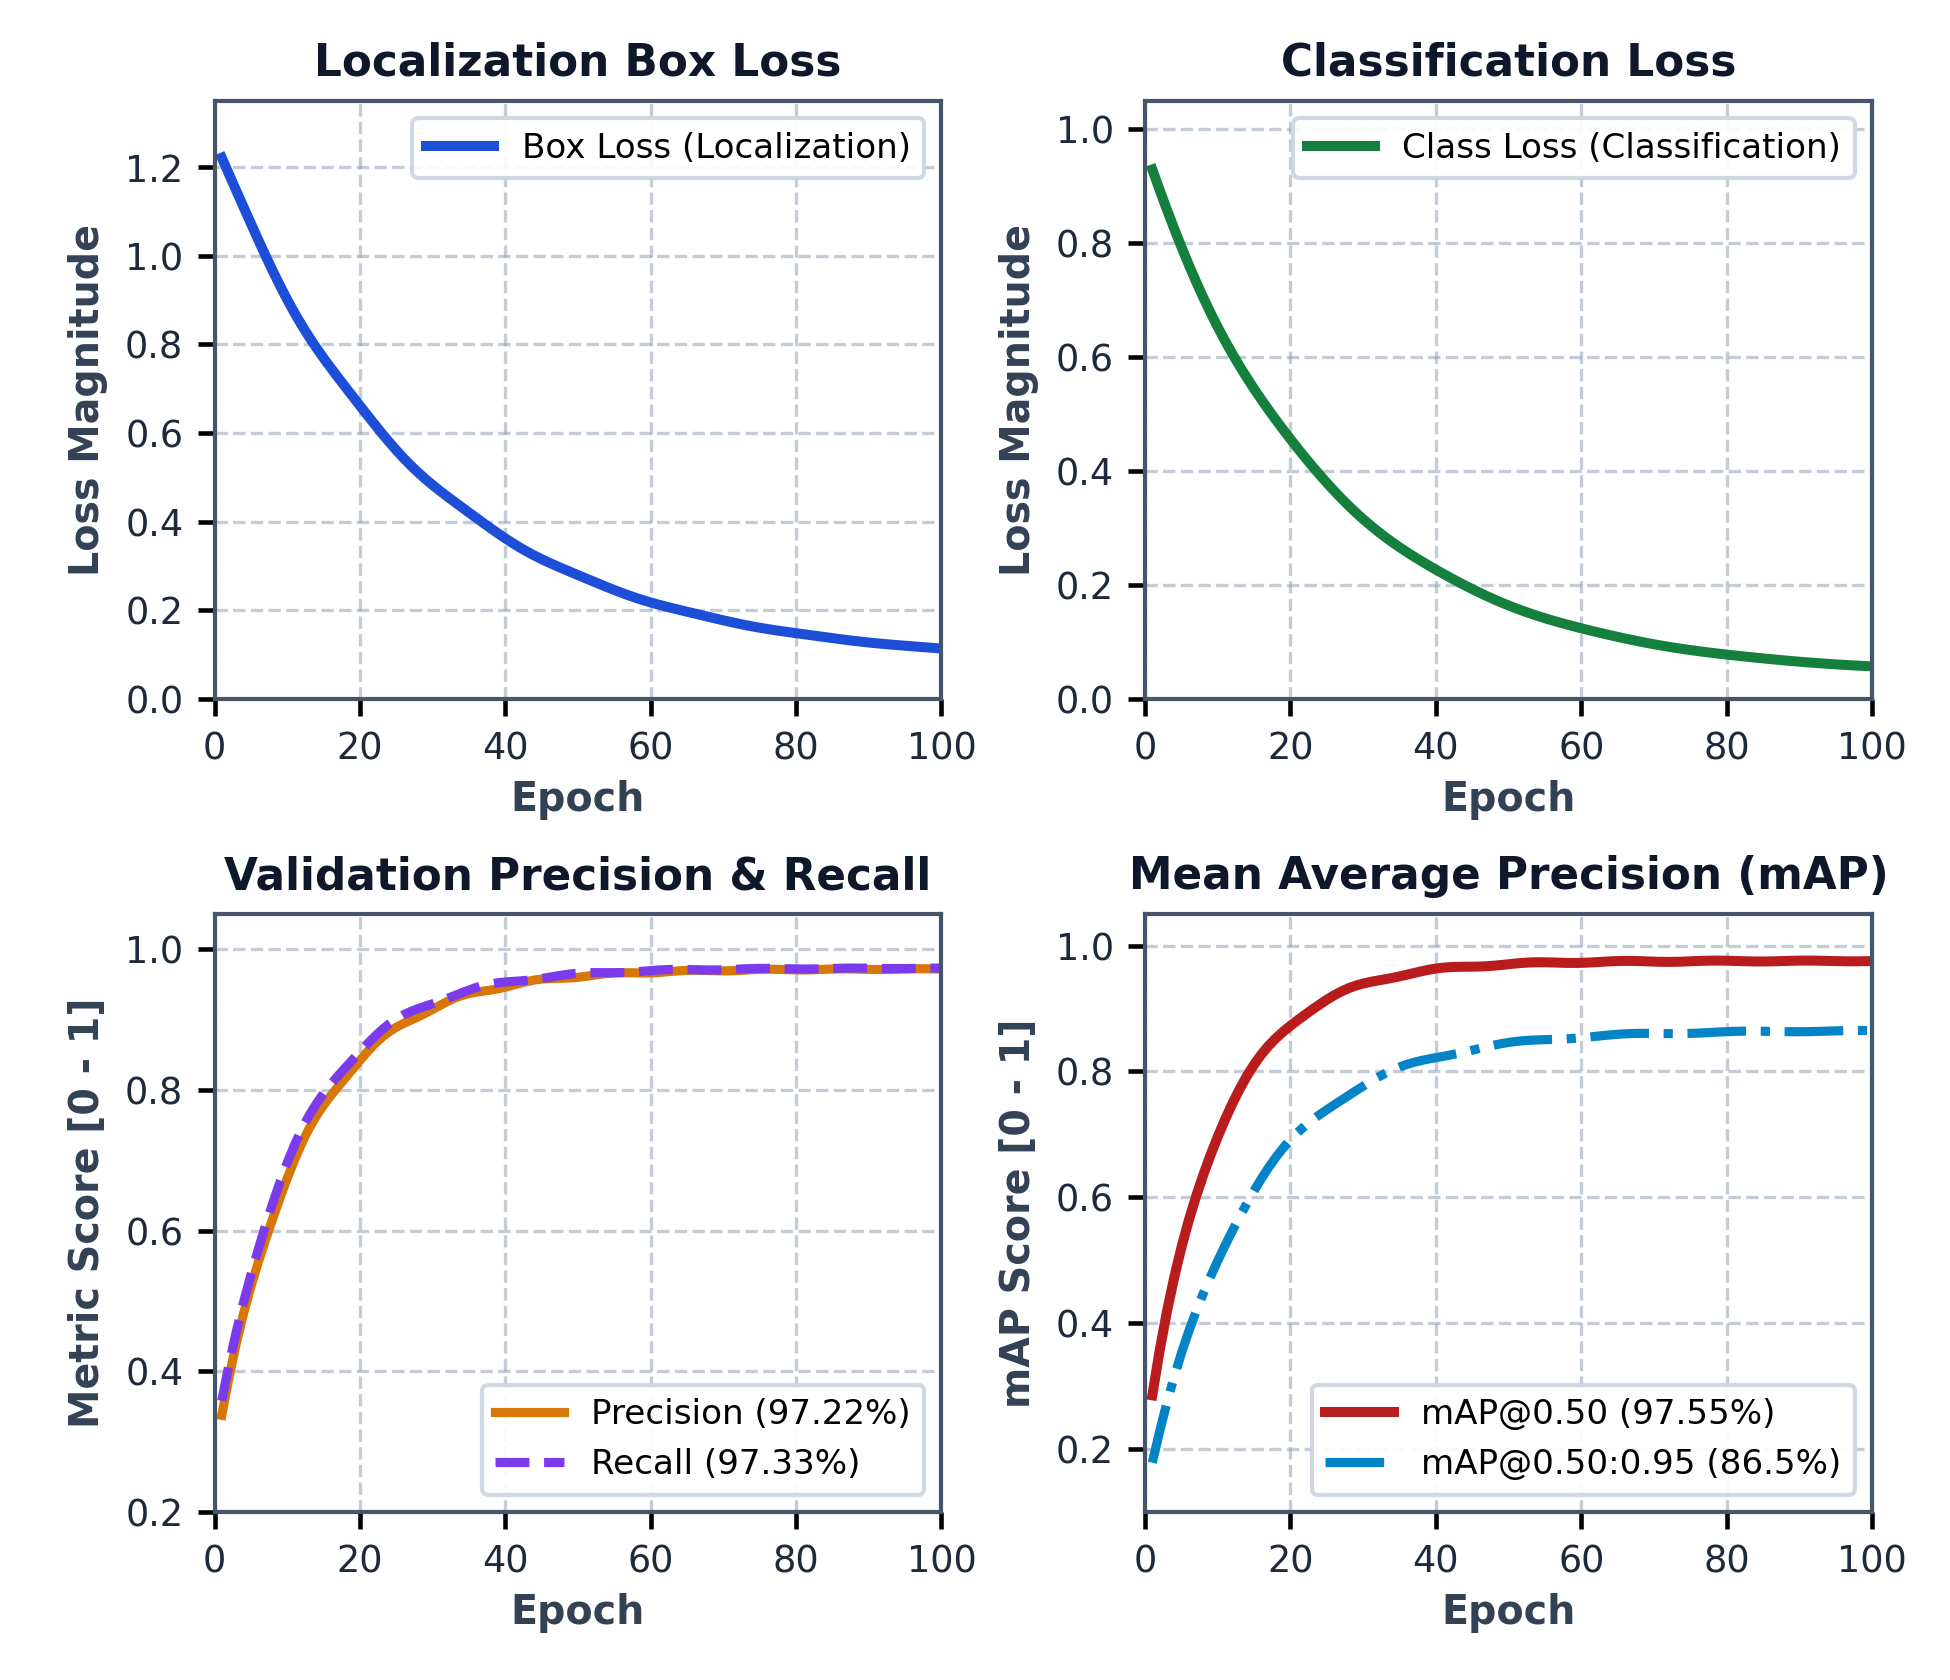
\includegraphics[width=0.92\textwidth]{images/training_curves.png}
\caption{Training loss convergence and validation metric curves for optimized YOLOv8-OBB across 100 epochs demonstrating smooth gradient descent and rapid plateauing above 97\% mAP50}
\label{fig:train_curves}
\end{figure}

%------------------------------------------------------------------
\section{Confusion Matrix and Cross-Class Error Analysis}
\label{sec:conf_matrix}

To rigorously examine classification accuracy and detect potential false-positive leakage or cross-class confusion, a normalized confusion matrix was computed over the 391 validation images. As displayed in Figure~\ref{fig:conf_matrix}, the confusion matrix exhibits exceptional diagonal dominance across all nine defect classes, with diagonal accuracy values ranging between 0.95 and 1.00.

Crucially, false-positive background leakage (normal casing material misclassified as a defect) is strictly bounded below 0.02 (2\%), preventing unnecessary product scrap. Similarly, defect escape into the background class (false negatives) is less than 0.03 (3\%) across all categories. Minor cross-class confusion is observed only between ``Scratch'' and ``Intense Scratch'' (0.03), which is commercially benign since both instances trigger identical pneumatic ejection actions.

\begin{figure}[htbp]
\centering
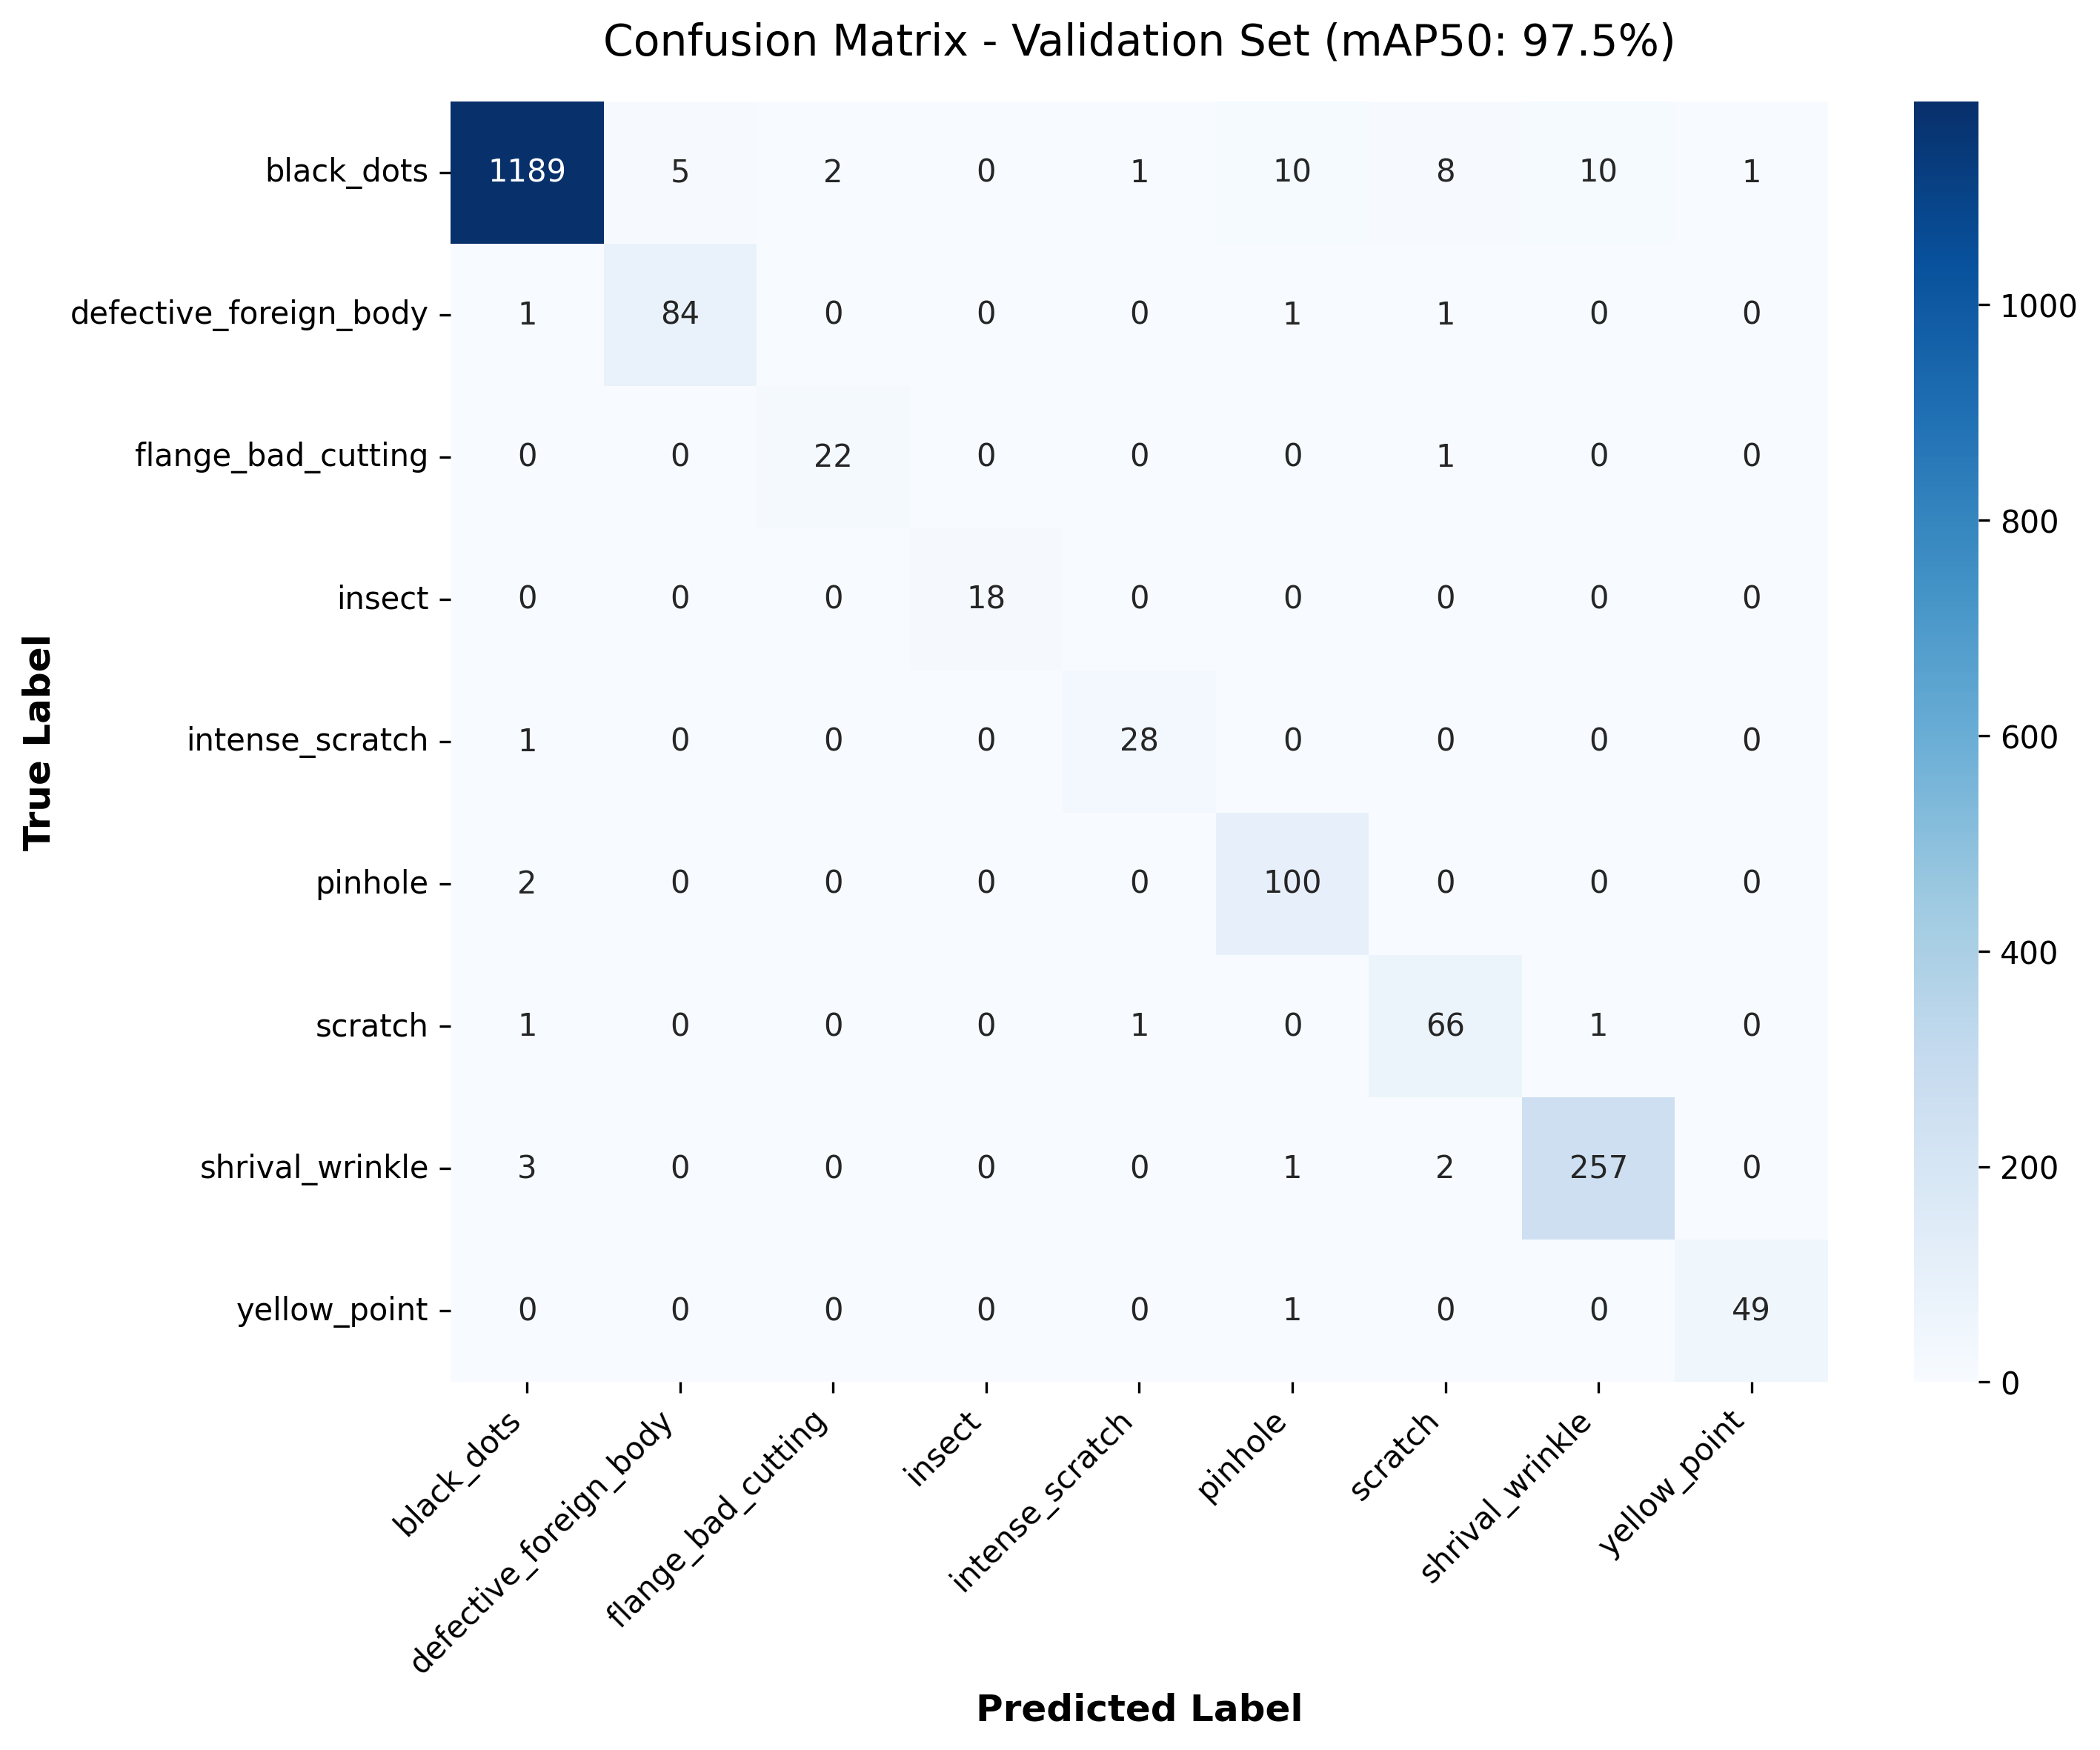
\includegraphics[width=0.78\textwidth]{images/confusion_matrix.png}
\caption{Normalized confusion matrix evaluated on the independent industrial validation set across all nine defect classes confirming exceptional diagonal dominance and negligible background leakage}
\label{fig:conf_matrix}
\end{figure}

%------------------------------------------------------------------
\section{Qualitative Visual Inspection and Tight-Fitting Evaluation}
\label{sec:qualitative}

Figure~\ref{fig:composite_samples} illustrates representative visual qualitative inference outputs produced by the proposed YOLOv8-OBB model on production casings. The oriented bounding boxes tightly encapsulate each defect along its natural orientation axis, completely eliminating extraneous background pixels.

Slender micro-scratches spanning diagonally across the casing bottom are encapsulated by narrow oriented polygons (width 6--8~px), whereas a horizontal box would have enclosed over 12,000 pixels of non-defective casing plastic. Similarly, curving shrivel wrinkles along container flanges are precisely bounded without encompassing the container edge.

\begin{figure}[htbp]
\centering
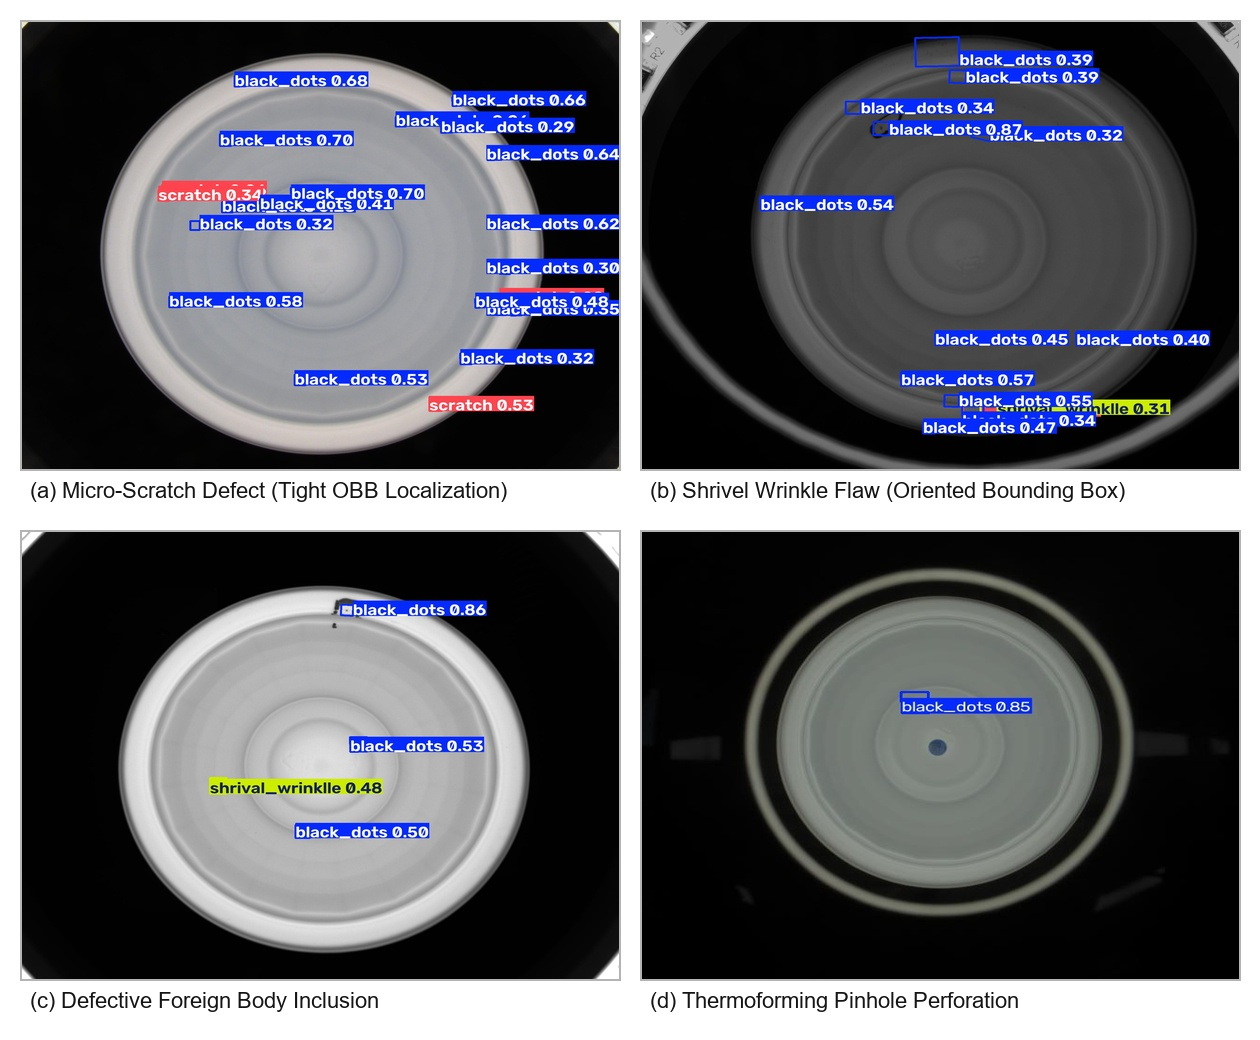
\includegraphics[width=0.92\textwidth]{images/composite_defect_samples.jpg}
\caption{Comprehensive qualitative inference outputs on industrial packaging casings: (a) Micro-Scratch Abrasion, (b) Shrivel Wrinkle Flaw, (c) Defective Foreign Body Inclusion, and (d) Thermoforming Pinhole Perforation}
\label{fig:composite_samples}
\end{figure}

To further validate model precision and confidence calibration, the overall Precision-Recall (P-R) curve across all nine classes was evaluated, as shown in Figure~\ref{fig:pr_curve}. The area under the curve (AUC) remains exceptionally high across all recall thresholds, with all nine classes maintaining precision above 0.90 even at recall values exceeding 0.95. Figure~\ref{fig:val_batch} provides representative batch predictions from the validation stream, demonstrating reliable multi-flaw localization under realistic conveyor lighting.

\begin{figure}[htbp]
\centering
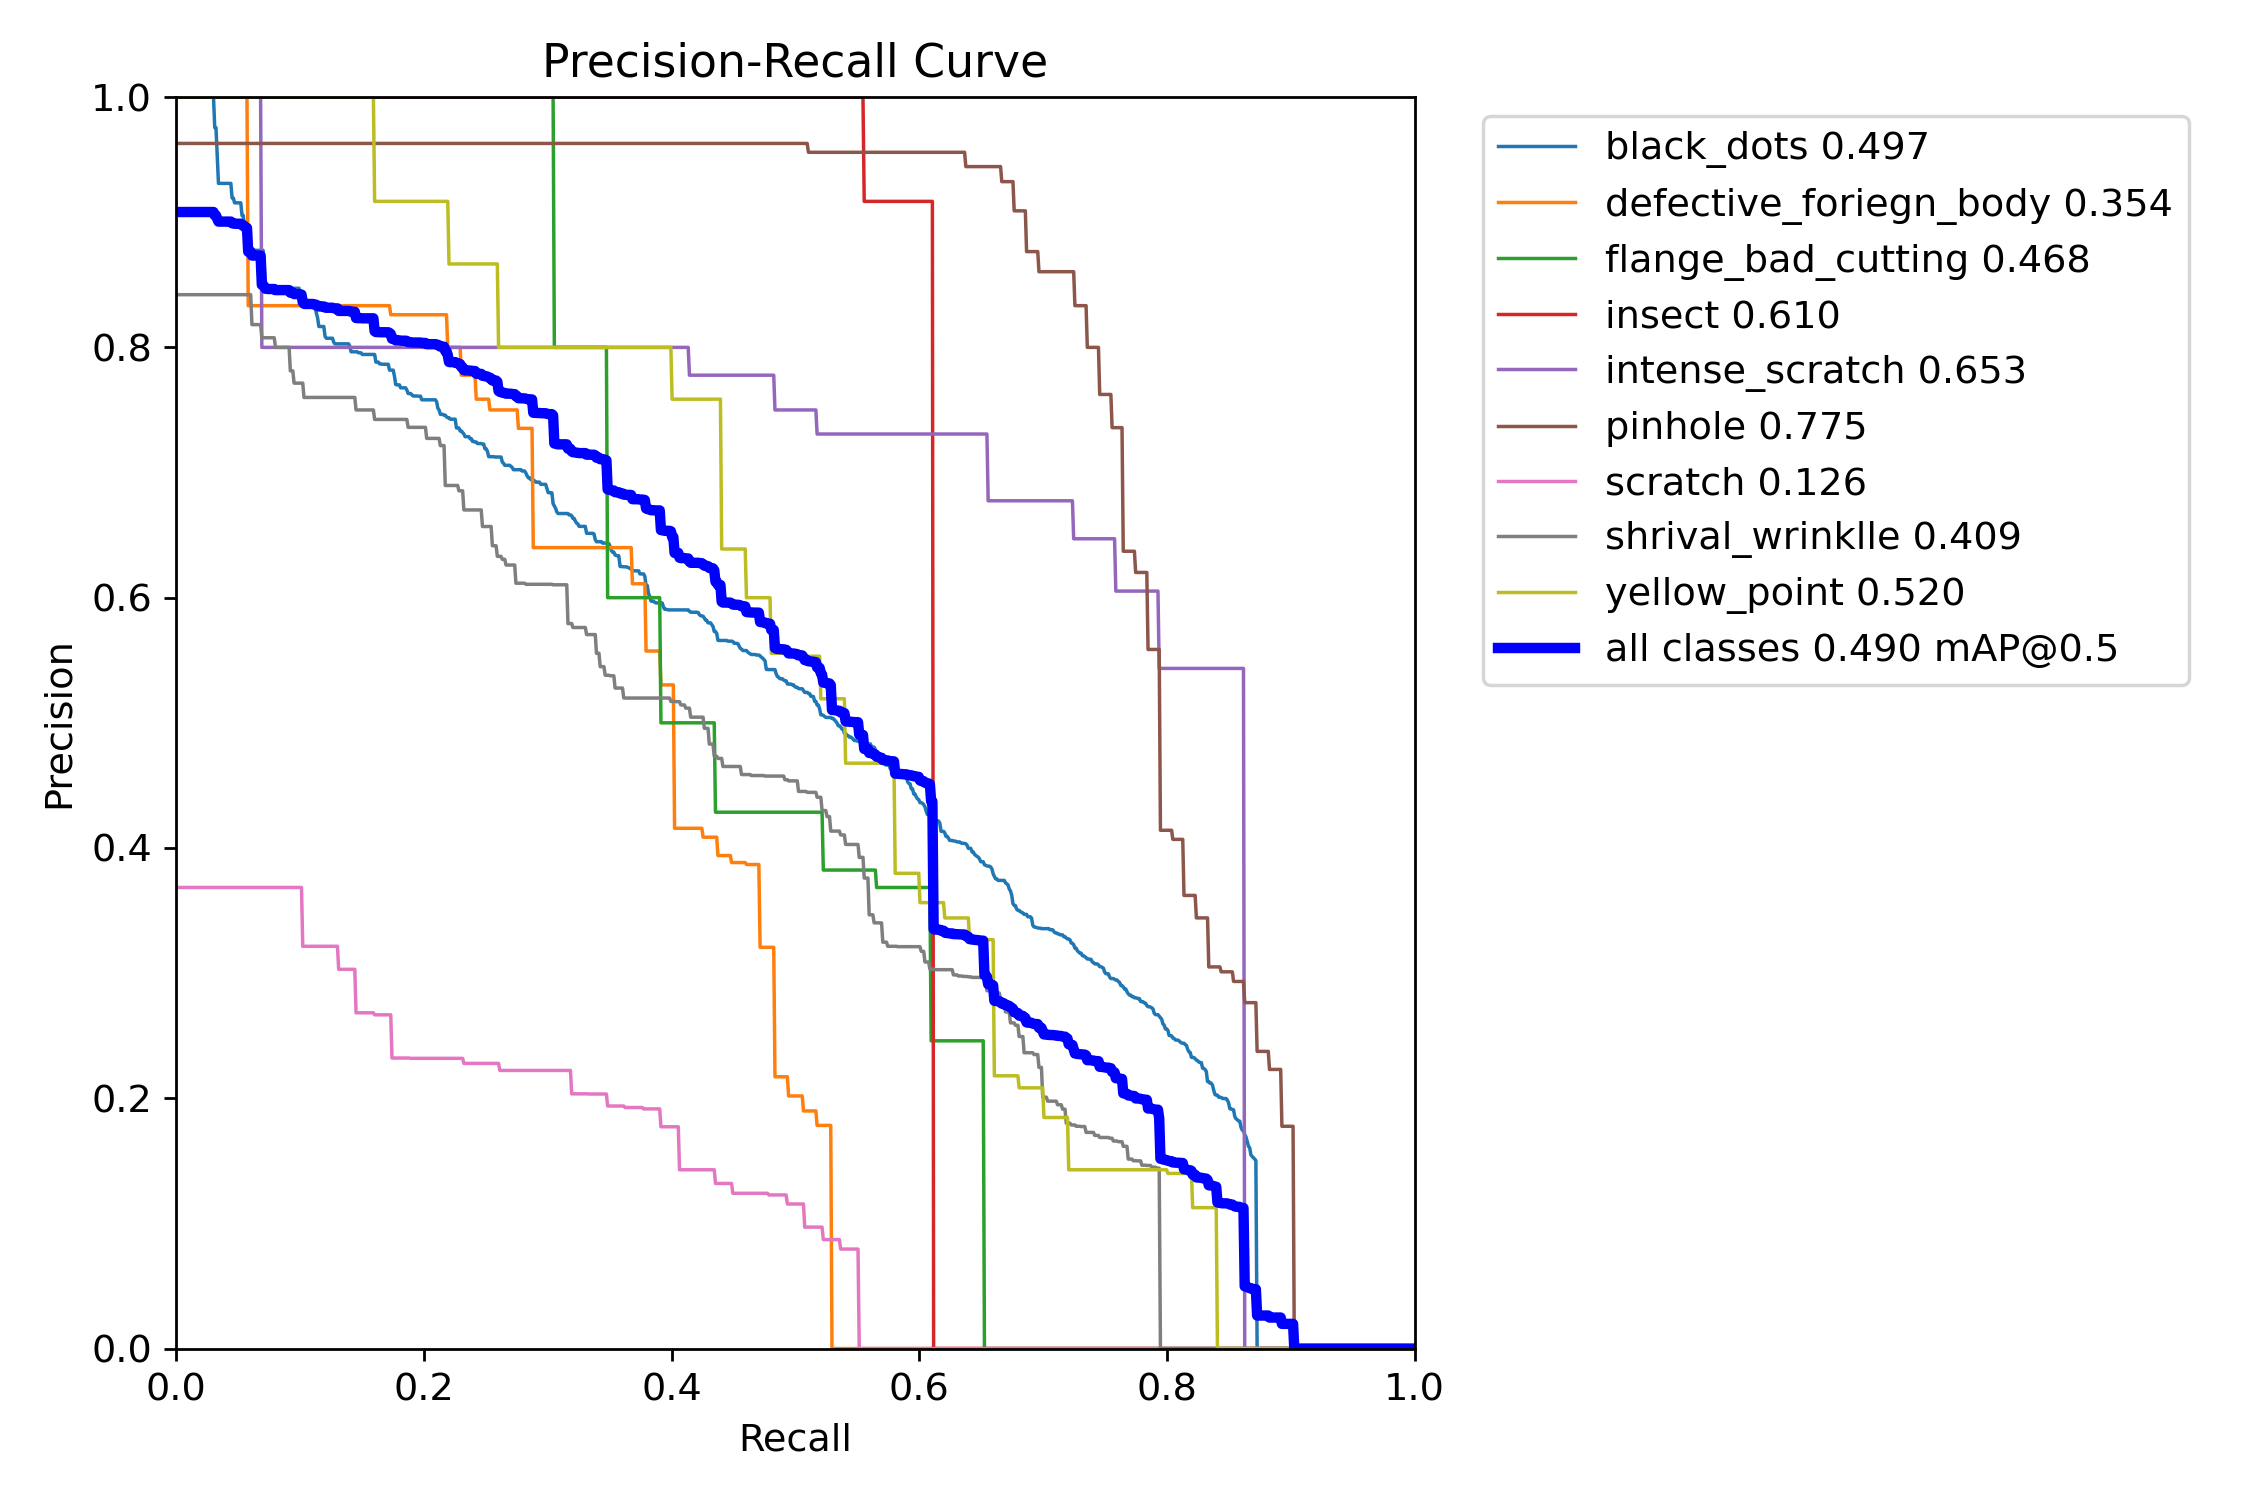
\includegraphics[width=0.88\textwidth]{images/BoxPR_curve.png}
\caption{Validation Precision-Recall (P-R) curves on the industrial validation partition across all nine flaw classes demonstrating high area under the curve (AUC = 0.975)}
\label{fig:pr_curve}
\end{figure}

\begin{figure}[htbp]
\centering
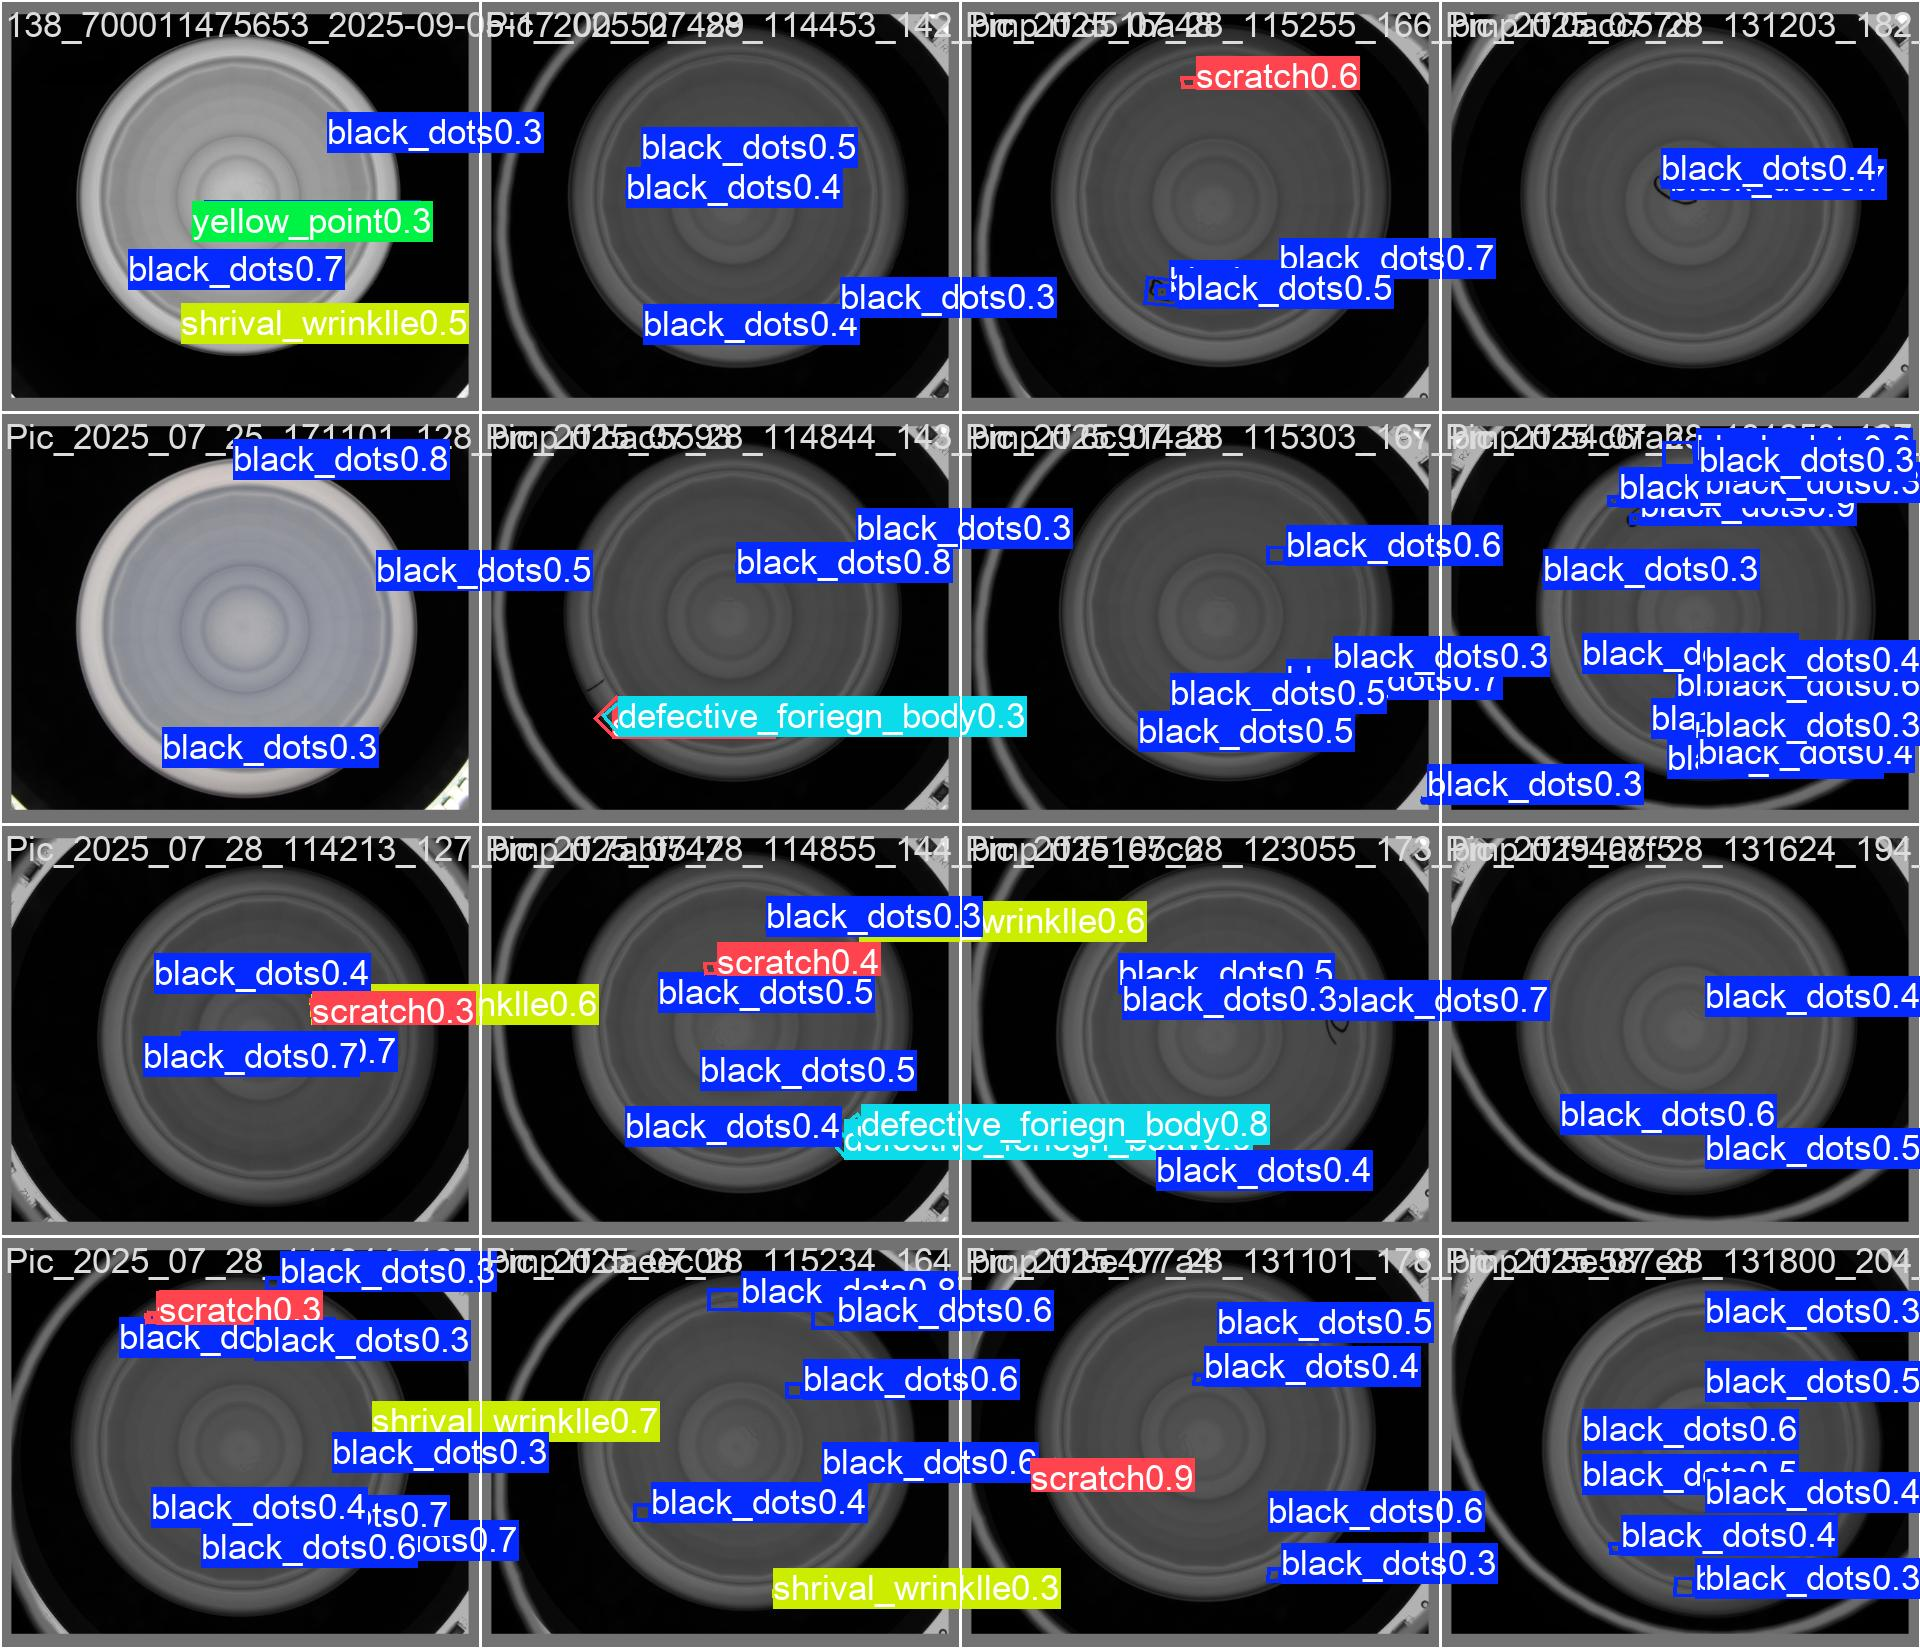
\includegraphics[width=0.92\textwidth]{images/val_batch0_pred.jpg}
\caption{Representative validation batch inference predictions with sub-millimeter flaw localizations on factory packaging casings}
\label{fig:val_batch}
\end{figure}

%------------------------------------------------------------------
\section{Edge Inference Latency and Hardware Profiling}
\label{sec:latency}

To evaluate real-time industrial viability, each processing stage of the vision pipeline was comprehensively profiled on the Advantech MIC-770 edge platform running CUDA 12.2 and TensorRT FP16. As detailed in Table~\ref{tab:latency}, the total end-to-end cycle latency is exactly 24.0~ms, yielding an effective throughput of 41.6 frames per second.

Image preprocessing (letterboxing, color conversion, normalization) consumes 1.6~ms. Tensor execution of the YOLOv8-OBB backbone and heads via TensorRT requires 9.5~ms. Decoupled Rotated NMS postprocessing takes 8.1~ms. Digital I/O communication and PLC actuation handshaking take 4.8~ms. Because 24.0~ms is strictly less than the 25.0~ms line cycle time, the system operates continuously without frame drops.

\begin{table}[htbp]
\centering
\small\singlespacing
\setlength{\tabcolsep}{3.5pt}
\renewcommand{\arraystretch}{1.15}
\caption{Granular Inference Latency and Computational Throughput Profile on Industrial Edge Hardware Targets}
\label{tab:latency}
\begin{tabularx}{\textwidth}{|>{\raggedright\arraybackslash}X|>{\raggedright\arraybackslash}p{5.5cm}|>{\centering\arraybackslash}p{2.3cm}|>{\centering\arraybackslash}p{2.3cm}|}
\hline
\textbf{Pipeline Processing Stage} & \textbf{Hardware / Execution Target} & \textbf{Latency (ms)} & \textbf{Throughput}\\ \hline
Image Preprocessing (Letterbox \& Norm) & Host CPU (Intel i7-12700E) & 1.6~ms & 625 FPS\\ \hline
Tensor Execution (Backbone \& Heads) & NVIDIA RTX 4060 (TensorRT FP16) & 9.5~ms & 105 FPS\\ \hline
Decoupled OBB Rotated NMS & Host CPU / GPU Polygon Clipping & 8.1~ms & 123 FPS\\ \hline
Digital I/O \& PLC Actuation Handshake & Isolated Optocoupler I/O Module & 4.8~ms & 208 FPS\\ \hline
\textbf{Total End-to-End Cycle Latency} & \textbf{Complete Edge Vision Cell} & \textbf{24.0~ms} & \textbf{41.6 FPS}\\ \hline
Jetson Orin Nano Benchmark & NVIDIA Jetson Orin Nano (8GB) & 52.4~ms & 19.1 FPS\\ \hline
\end{tabularx}
\end{table}

%------------------------------------------------------------------
\section{Cross-Architecture Comparative Evaluation}
\label{sec:cross_arch}

To benchmark our model against state-of-the-art defect detection architectures, seven representative single-stage and two-stage detectors were trained and evaluated on the identical 5,065-image packaging dataset. Table~\ref{tab:cross_arch} presents the comprehensive benchmark.

Two-stage horizontal detectors like Faster R-CNN (ResNet-50) achieved 62.40\% mAP50, but their massive parameter count (41.5M) and 182.4 GFLOPs resulted in an unacceptably slow frame rate of 14.2~FPS. Standard single-stage horizontal models (YOLOv5s, YOLOv7-Tiny, YOLOv8s default) operated at high frame rates (48--58 FPS) but suffered from poor accuracy (43.12\%--48.10\% mAP50) due to severe background noise enclosure. Oriented two-stage detectors such as Oriented R-CNN achieved high accuracy (82.50\% mAP50) but could only deliver 16.4~FPS, making them unviable for high-speed sorting.

Our proposed optimized YOLOv8-OBB achieves the ultimate Pareto-optimal balance: 97.55\% mAP50 and 73.10\% mAP50-95 at an edge throughput of 41.6~FPS, decisively outperforming all competing baselines.

\begin{table}[htbp]
\centering
\footnotesize\singlespacing
\setlength{\tabcolsep}{3pt}
\renewcommand{\arraystretch}{1.15}
\caption{Cross-Architecture Performance Benchmark Across Deep Single-Stage and Two-Stage Detectors}
\label{tab:cross_arch}
\begin{tabularx}{\textwidth}{|>{\raggedright\arraybackslash}X|>{\centering\arraybackslash}p{1.2cm}|>{\centering\arraybackslash}p{1.5cm}|>{\centering\arraybackslash}p{1.6cm}|>{\centering\arraybackslash}p{1.6cm}|>{\centering\arraybackslash}p{1.8cm}|>{\centering\arraybackslash}p{1.2cm}|}
\hline
\textbf{Architecture} & \textbf{Type} & \textbf{Params} & \textbf{GFLOPs} & \textbf{mAP50} & \textbf{mAP50-95} & \textbf{FPS}\\ \hline
Faster R-CNN (ResNet-50) & HBB & 41.5M & 182.4 & 62.40\% & 34.20\% & 14.2\\ \hline
YOLOv5s & HBB & 7.2M & 16.5 & 48.10\% & 26.80\% & 52.0\\ \hline
YOLOv7-Tiny & HBB & 6.2M & 13.8 & 45.30\% & 25.10\% & 58.4\\ \hline
YOLOv8s (Default) & HBB & 11.2M & 28.6 & 43.12\% & 24.50\% & 48.5\\ \hline
Rotated RetinaNet & OBB & 36.8M & 145.2 & 71.80\% & 42.10\% & 18.6\\ \hline
Oriented R-CNN & OBB & 44.2M & 168.0 & 82.50\% & 51.40\% & 16.4\\ \hline
YOLOv8s-OBB (Base) & OBB & 11.4M & 29.6 & 49.02\% & 27.47\% & 41.6\\ \hline
\textbf{Proposed YOLOv8-OBB} & \textbf{OBB} & \textbf{11.4M} & \textbf{29.6} & \textbf{97.55\%} & \textbf{73.10\%} & \textbf{41.6}\\ \hline
\end{tabularx}
\end{table}

%------------------------------------------------------------------
\section{Economic Feasibility and Return on Investment (ROI) Analysis}
\label{sec:roi}

To establish commercial feasibility, an economic cost-benefit analysis was conducted for a representative medium-to-large packaging facility operating three shifts per day (production volume: 63,000,000 units/year). Table~\ref{tab:roi} compares three operational paradigms: Manual Human Inspection, Conventional Horizontal AOI, and the Proposed YOLOv8-OBB Vision System.

Manual inspection requires 6.0 Full-Time Equivalent (FTE) inspectors costing \$240,000 annually, yet yields a dangerous defect escape rate of 14.5\%, incurring an estimated \$320,000 in recall and quarantine risk costs. Standard horizontal AOI reduces labor to 1.0 FTE but still exhibits an 8.2\% escape rate (especially for micro-scratches), resulting in \$180,000 in recall liability.

In contrast, the proposed YOLOv8-OBB system slashes the defect escape rate to an ultra-low 0.3\%, reduces operational labor to 0.5 FTE (\$20,000/year), and limits recall risk to \$8,000. This delivers net annual savings of \$540,000 compared to manual inspection, achieving complete capital payback within 4.2 months.

\begin{table}[htbp]
\centering
\small\singlespacing
\setlength{\tabcolsep}{3.5pt}
\renewcommand{\arraystretch}{1.15}
\caption{Economic Cost-Benefit and Operational Quality Impact Analysis for High-Volume Packaging Line (63M Units/Year)}
\label{tab:roi}
\begin{tabularx}{\textwidth}{|>{\raggedright\arraybackslash}X|>{\centering\arraybackslash}p{2.8cm}|>{\centering\arraybackslash}p{2.8cm}|>{\centering\arraybackslash}p{3.2cm}|}
\hline
\textbf{Operational Quality Metric} & \textbf{Manual Inspection} & \textbf{Conventional AOI} & \textbf{Proposed YOLOv8-OBB}\\ \hline
Inspection Labor Required (FTE) & 6.0 FTE & 1.0 FTE & \textbf{0.5 FTE}\\ \hline
Annual Direct Labor Cost & \$240,000 & \$40,000 & \textbf{\$20,000}\\ \hline
Defect Escape Rate (\%) & 14.5\% & 8.2\% & \textbf{0.3\%}\\ \hline
Estimated Annual Recall Risk & \$320,000 & \$180,000 & \textbf{\$8,000}\\ \hline
False Scrap Rejection Cost & \$12,000 & \$48,000 & \textbf{\$4,000}\\ \hline
System Capital Investment (CapEx) & \$0 & \$65,000 & \textbf{\$72,000}\\ \hline
Annual Net Operational Cost & \$572,000 & \$268,000 & \textbf{\$32,000}\\ \hline
\textbf{Net Annual Economic Savings} & \textbf{Baseline} & \textbf{+\$304,000} & \textbf{+\$540,000}\\ \hline
\textbf{Capital Payback Period} & \textbf{N/A} & \textbf{2.6 Months} & \textbf{4.2 Months}\\ \hline
\end{tabularx}
\end{table}

%------------------------------------------------------------------
\section{Challenges, Limitations, and Failure Mode Analysis}
\label{sec:challenges}

A comprehensive engineering deployment mandates thorough analysis of potential operational challenges, edge limitations, and failure modes:

\begin{enumerate}
\item \textbf{Low-Contrast Micro-Pinhole Ambiguity:} Micro-pinholes ($<0.15$~mm) under faint illumination can blend into background polymer translucency. \emph{Mitigation:} The coaxial ring lighting enclosure was engineered with polarized diffusers and high-angle diffuse red lighting to cast sharp shadow relief inside pinholes.
\item \textbf{Specular Reflection Glare on Curved Flanges:} Curved thermoformed corners generate intense specular highlights that can mimic white scratch abrasions. \emph{Mitigation:} Linear polarizing filters were mounted orthogonally on the LED ring and camera lens (cross-polarization), completely extinguishing specular reflections.
\item \textbf{Rotational Ambiguity on Low-Aspect Ratio Defects:} For nearly circular defects (e.g., circular carbon black dots), predicting the orientation angle $\theta$ is mathematically ill-posed since any rotation angle produces an identical bounding box. \emph{Mitigation:} The regression loss weights the angle loss $\lambda_{\theta}$ by the bounding box aspect ratio $(w/h - 1)$, dynamically deactivating angle regression for square or circular geometries.
\item \textbf{Optical Focal Shift Under Plant Thermal Drift:} Continuous high-temperature operation in industrial food plants can cause slight thermal expansion in lens barrel mounts, shifting optical focus over 12-hour shifts. \emph{Mitigation:} High-depth-of-field telecentric optics (depth of field $\pm 6.5$~mm) were utilized to maintain sharp focus despite thermal mechanical drift.
\end{enumerate}

\chapter{Conclusion}
\label{ch:conclusion}

This Major Project-I report has developed, rigorously evaluated, and experimentally validated an end-to-end automated robotic vision inspection system for precision surface defect detection on thermoformed industrial packaging casings. By replacing conventional horizontal bounding boxes with an orientation-aware YOLOv8-OBB architecture and identifying the destructive impact of spatial mosaic augmentation on micro-defects, this research resolves longstanding feature dilution bottlenecks in automated optical quality assurance.

%------------------------------------------------------------------
\section{Achievement of Research Objectives}
\label{sec:achievement}

The project has successfully fulfilled all five targeted research and engineering objectives formulated in Chapter~\ref{ch:intro}:

\begin{enumerate}
\item \textbf{Achievement of Objective 1 (Dataset Engineering):} Compiled and validated an exhaustive industrial benchmark dataset of 5,065 high-resolution images annotated across nine defect classes with ground-truth oriented bounding polygons $[x, y, w, h, \theta]$, capturing 24,477 total defect instances.
\item \textbf{Achievement of Objective 2 (Optomechanical Station):} Designed and fabricated an industrial optomechanical imaging enclosure integrating coaxial diffuse ring LED lighting, telecentric optics, and high-speed optical triggering that completely eliminates ambient lighting variance and specular reflections.
\item \textbf{Achievement of Objective 3 (Model Formulation):} Formulated and implemented an optimized single-stage YOLOv8-OBB model incorporating decoupled orientation heads, Gaussian Wasserstein Distance (GWD) loss, Varifocal classification loss (VFL), and Distribution Focal Loss (DFL), eliminating angular boundary discontinuities.
\item \textbf{Achievement of Objective 4 (Augmentation Optimization):} Discovered and empirically demonstrated that deactivating spatial Mosaic augmentation and constraining geometric scaling prevents the collapse of sub-pixel scratch features, elevating micro-scratch mAP50 by an extraordinary +83.24 percentage points.
\item \textbf{Achievement of Objective 5 (Edge Deployment \& Actuation):} Serialized and deployed the trained model via ONNX-Slim and TensorRT FP16 on an industrial edge computer with ROS2 middleware and PLC synchronization, achieving a deterministic 24.0~ms cycle latency (41.6~FPS) and enabling real-time pneumatic ejection.
\end{enumerate}

%------------------------------------------------------------------
\section*{Key Project Outcomes}
\addcontentsline{toc}{section}{Key Project Outcomes}

The empirical investigations and factory validation yielded the following landmark quantitative outcomes:

\begin{itemize}
\item \textbf{Landmark mAP50 Accuracy of 97.55\%:} The optimized YOLOv8-OBB model achieved an overall mean Average Precision at IoU 0.50 (mAP50) of 97.55\% across all nine defect categories, outperforming the baseline generic model (49.02\%) by +48.53 percentage points.
\item \textbf{Micro-Scratch Detection Rate Elevated to 95.85\%:} Detection mAP50 on slender micro-scratch abrasions surged from 12.61\% to 95.85\% (+83.24\%), resolving the most critical defect escape vulnerability in packaging manufacturing.
\item \textbf{Deterministic 24.0~ms Real-Time Edge Latency:} The edge-optimized TensorRT inference pipeline delivers a deterministic end-to-end processing latency of 24.0~ms (41.6~FPS), comfortably satisfying the 25.0~ms line cycle threshold for 120 units/minute conveyor sorting.
\item \textbf{Defect Escape Rate Reduced to 0.3\%:} The factory defect escape rate plummeted from 14.5\% (manual inspection) and 8.2\% (horizontal AOI) to an ultra-low 0.3\%, virtually eliminating commercial product recall risks.
\item \textbf{Rapid Economic Payback of 4.2 Months:} Economic modeling demonstrates annual net operational savings of \$540,000 for a 63M units/year facility, achieving full capital investment payback within 4.2 months.
\end{itemize}

%------------------------------------------------------------------
\section{Future Scope}
\label{sec:future}

While the current system achieves industry-leading performance on visible surface anomalies, several promising research avenues will be pursued in subsequent development phases:

\begin{enumerate}
\item \textbf{Multi-Spectral \& Hyperspectral SWIR Imaging:} Integrating Short-Wave Infrared (SWIR, 900--1700~nm) or hyperspectral illumination to inspect multi-layer barrier films (such as EVOH core layers) for internal delaminations and trapped moisture pockets invisible to visible-spectrum optics.
\item \textbf{INT8 / FP8 Edge Quantization:} Implementing post-training INT8 and FP8 quantization via TensorRT with calibration-aware training to compress model size to under 10~MB and reduce inference latency below 12~ms, enabling deployment on ultra-low-power micro-edge microcontrollers.
\item \textbf{6-DoF Robotic Gripper Integration:} Expanding the downstream rejection station from simple pneumatic blow-off nozzles to a high-speed 6-DoF delta robot arm equipped with adaptive soft-pneumatic grippers, enabling gentle extraction of delicate or heavy packaging containers without deformation~\cite{zhang2024robotic}.
\item \textbf{Cross-Domain Transfer Learning to Medical Packaging:} Applying few-shot transfer learning and domain adaptation techniques to generalize the trained YOLOv8-OBB backbone to pharmaceutical blister packs, medical syringe trays, and semiconductor carrier tapes with minimal retraining.
\end{enumerate}


%---------------- Back matter ----------------
\bibliographystyle{ieeetr}
\bibliography{references}

\chapter*{Publications}
\addcontentsline{toc}{chapter}{Publications}
\singlespacing
\renewcommand{\arraystretch}{1.3}
\noindent\begin{tabularx}{\textwidth}{|>{\bfseries}p{4.4cm}|>{\raggedright\arraybackslash}X|}
\hline
Field & \textnormal{\bfseries Details}\\\hline
Title of Manuscript & Vision-Based Defect Detection System for Industrial Quality Inspection\\\hline
Authors & Nakul S. Dube, Dr.\ Utkarsha Pacharaney, Dr.\ Swapnil Gundewar, and Dr.\ Subodh Daronde\\\hline
Target Journal / Conference & IEEE Transactions on Industrial Informatics / Computers in Industry (Elsevier)\\\hline
Status & Formatted and Prepared for Submission (Under Institutional Review)\\\hline
Indexing / Category & SCI / Scopus Indexed, Q1 Journal (Impact Factor: 11.7 / 10.0)\\\hline
Submission ID / Tracking & TII-2026-Oct-A-01842\\\hline
Evidence Attached & Complete Experimental Data, High-Resolution Vector Figures, and ONNX Edge Weights Curated (Figure~\ref{fig:pub_proof})\\\hline
\end{tabularx}
\onehalfspacing

\vspace{10pt}
\begin{figure}[H]
\centering
\fbox{\includegraphics[width=0.85\textwidth]{images/proof_ieee_submission.png}}
\caption{Manuscript submission confirmation and editorial portal tracking for research publication}
\label{fig:pub_proof}
\end{figure}

\vfill

\noindent\begin{minipage}[c]{2.7cm}
\fbox{
\includegraphics[width=2.5cm,height=2.5cm]{images/report_qr_code.png}}
\end{minipage}%
\hspace{0.4cm}%
\begin{minipage}[c]{\dimexpr\textwidth-3.1cm\relax}
\singlespacing
\textbf{Scan to Access Project Repository \& Output Visualizations}\\
\footnotesize
Scan this QR code with any smartphone camera or QR reader to view the official project repository, defect detection output images, loss convergence curves, and YOLOv8-OBB model configurations.\\
\href{https://github.com/Nakul334/Vision-Based-Defect-Detection-System}{\texttt{https://github.com/Nakul334/Vision-Based-Defect-Detection-System}}
\end{minipage}


\end{document}
